\chapter{نتایج عملی} \label{chap:experiments}
در این فصل، روش‌های پیشنهادی را روی چند مجموعه دادگان آزمایش کرده و نتایج آن را با سایر روش‌های ارائه شده برای یادگیری بدون نمود نمونه‌ای مقایسه می‌کنیم. در این فصل ابتدا مجموعه دادگان مورد استفاده در آزمایشات معرفی می‌شوند. سپس کارایی روش‌های ارائه شده در بخش‌های
\ref{nn}
تا
\ref{jeac}
با آزمایش روی این مجموعه دادگان مورد بررسی قرار می‌گیرد و تاثیر هر قسمت‌های مختلف هر یک از روش‌های پیشنهادی و پارامترهای موجود در آن‌ها سنجیده می‌شود.


\section{مجموعه دادگان مورد استفاده}\label{exp:datasets}
برای آزمایشات عملی ما از چهار مجموعه داده‌ی مرسوم برای سنجش عمل‌کرد روش‌های یادگیری بدون نمود نمونه‌ای استفاده می‌کنیم.

\textbf{\lr{Animal with Attributes (AwA)}} \cite{lampert09}:
این مجموعه داده شامل تصاویری از ۵۰ گونه از پستانداران است. هر دسته توسط یک بردار صفت $-85$بعدی توصیف می‌شود. در این مجموعه داده توصیف‌های دسته‌ها هم به صورت مقادیر دودویی به معنای وجود یا عدم وجود آن صفت وجود دارند و هم توسط اعداد حقیقی با توجه به میزان وجود آن صفت در هر دسته در دسترس هستند. در آزمایش‌های انجام شده از مقادیر پیوسته برای توصیف دسته‌ها استفاده شده است، چرا که در روش‌های پیشین نشان داده شده که این مقادیر توانای ایجاد تمایز بیشتری دارند \cite{Akata2015}. هم‌چنین از تقسیم‌بندی آموزش و آزمون انجام شده در خود مجموعه داده استفاده می‌کنیم که در آن ۴۰ دسته به عنوان دسته‌های دیده شده و ۱۰ دسته به عنوان
دسته‌های دیده نشده در نظر گرفته شده‌اند.

\textbf{\lr{aPascal/aYahoo (aPY)}}\cite{farhadi09}:
مجموعه تصاویر
 \lr{VOC 2008} \cite{pascal}
 که شامل ۲۰ دسته است بعنوان دسته‌های دیده شده در نظر گرفته شده است و تصاویر \lr{aYahoo} که شامل ۱۲ دسته هستند به عنوان دسته‌های دیده نشده. برای این دو مجموعه داده، بردار صفت‌های $-64$بعدی دودویی برای هر تصویر موجود است. برای بدست آوردن توصیف هر دسته که در مسئله یادگیری بدون نمود نمونه‌ای مورد نیاز است، همانند روش‌های پیشین، روی بردار صفت‌های تصاویر هر دسته میان گرفته
 شده است  \cite{lampert09}.


\textbf{\lr{SUN Attribute}} \cite{sun}:
مجموعه تصاویر SUN شامل ۷۱۷ دسته می‌باشد و در این مجموعه برای هر یک از تصاویر یک بردار صفت $-102$بعدی موجود است که برای تبدیل آن به توصیف‌های در سطح دسته‌ها، روی بردار صفت‌های تصاویر هر دسته میانگین گرفته شده است. ما تقسیم‌بندی آموزش/آزمون انجام گرفته در \cite{jayaraman14} استفاده می‌کنیم که در آن ۱۰ دسته به عنوان دسته‌های دیده نشده در نظر گرفته شده‌اند.

\textbf{\lr{Caltech UCSD Birds-2011 (CUB)}} \cite{cub}:
این مجموعه داده شامل تصاویری از ۲۰۰ گونه از پرندگان است. هر تصویر با ۳۱۲ صفت دودویی توصیف می‌شود و توصیف در نظر گرفته شده برای هر دسته میانگین توصیف نمونه‌های آن دسته است. تقسیم‌بندی مورد استفاده برای دسته‌های آموزش و آزمون، دسته‌بندی مورد استفاده در \cite{akata13} است که توسط کارهای بعدی نیز مورد استفاده قرار گرفته است
\cite{sse, Akata2015, Reed2016}.


در تمام مجموعه داده‌ها، برای تصاویر از ویژگی‌های بدست آمده با شبکه‌های ژرف استفاده می‌کنیم چرا که توانایی ایجاد تمایز این ویژگی‌ها نسبت به ویژگی‌های
\textit{کم‌عمق}
سنتی مانند \lr{SIFT}  و \lr{HOG}  بیشتر است.
ویژگی‌های مورد استفاده از  اولین لایه با اتصالات چگال از شبکه ۱۹ لایه‌ی \lr{VGG} \cite{vgg} بدست آمده است. پیش آموزش شبکه  روی زیرمجموعه‌ای از
مجموعه دادگان ImageNet
\cite{imagenet}
مربوط به چالش سال ۲۰۱۲ دسته‌بندی تصاویر در مقیاس بالا
\LTRfootnote{ImageNet Large Scale Visual Recognition Challenge (ILSVRC12)}
 \cite{ILSVRC15} انجام شده است.
 این تصاویر شامل ۱۵۰۰۰۰ تصویر از ۱۰۰۰ دسته هستند.
 این ویژگی‌ها به صورت عمومی توسط نویسندگان
\cite{sse}
در اختیار قرار گرفته است.

مشخصات مجموعه دادگان مورد استفاده به صورت خلاصه در جدول \ref{tab:datasets} آمده است.
\begin{center}

\begin{table}[ht]
\centering
\caption{مشخصات مجموعه دادگان مورد استفاده در آزمایشات عملی}
\vspace{2mm}
\label{tab:datasets}
\begin{tabular}{|r|c|c|c|c|c|c|}
\hline
 مجموعه داده & ابعاد توصیف‌ & ابعاد تصاویر &  دسته‌های آموزش & دسته‌های آزمون &  نمونه‌های آموزش &  نمونه‌های آزمون \\
\hline
AwA
& 85 & 4096 & 40 & 10 & 24295 & 6180 \\\hline
 aPY
& 64 & 4096 & 20 & 12 & 12695 & 2644 \\\hline
CUB-2011
& 312 & 4096 & 150 & 50 & 8855 & 2933 \\ \hline
 SUNA
& 102 & 4096 & 707 & 10 & 14140 & 200 \\
\hline
\end{tabular}
\end{table}
\end{center}
%
\section{نحوه‌ی اعتبارسنجی}\label{exp:validation}
برای تعیین پارامترهای مورد استفاده در روش‌های ارائه شده،  از یک الگوریتم اعتبار سنجی مرسوم در روش‌های یادگیری بدون نمود نمونه‌ای استفاده می‌شود.
پارامترهای موجود در روش‌ها عبارتند از:
\begin{itemize}
\item
 \gls{hyperparameter} $\gamma$ در رابطه \eqref{eq:nn_loss}. این \gls{hyperparameter} که در شبکه عصبی چندوظیفه‌ای پیشنهاد شده به کار رفته و نشان‌دهنده میزان تاثیر نمونه‌های آزمون در تابع هزینه است.
\item
مقدار $\alpha$ در رابطه \eqref{eq:d_definition} که وزن جمله‌ی منظم‌سازی را در یادگیری نگاشت از فضای توصیف دسته‌ها به فضای تصاویر تعیین می‌کند.
\item
مقادیر  $\lambda$ و $\eta$ در رابطه \eqref{eq:joint} که به ترتیب میزان اهمیت جمله مربوط به نمونه‌های آزمون و وزن جمله‌ی منظم‌سازی را در یادگیری نگاشت از فضای توصیف دسته‌ها به فضای تصاویر  تعیین می‌کنند.
\end{itemize}
در این شیوه‌ی اعتبار سنجی تعدادی از دسته‌های آموزش به عنوان دسته‌های اعتبارسنجی در نظر گرفته شده و اعتبار سنجی به این صورت انجام می‌شود که آموزش روی سایر دسته‌ها صورت گرفته و روی دسته‌های اعتبارسنجی که دیده نشده فرض شده‌اند، سنجیده می‌شود. بدیهی است که مجموعه‌ دسته‌های آزمون اصلی در این روند به هیچ صورتی مورد استفاده قرار نمی‌گیرند. وقتی مقادیر پارامترها تعیین شد، روش روی کل دسته‌های دیده‌شده آموزش می‌بیند. ما تعداد دسته‌های اعتبارسنجی را برای هر مجموعه به گونه‌ای انتخاب کردیم که نسبت تعداد دسته‌های اعتبارسنجی به سایر دسته‌های آموزش برابر نسبت تعداد دسته‌های آزمون به کل دسته‌های آموزش باشد. برای اعتبار سنجی الگوریتم به ازای هر مقدار پارامتر ۱۰ بار با انتخاب تصادفی دسته‌های اعتبارسنجی از دسته‌های آزمون اجرا شده و عمل‌کرد روی این ۱۰ حالت میانگین گرفته شده است.
%
\section{معیار سنجش روش‌ها}\label{criteria}
 معیار مورد استفاده برای این مقایسه که پرکاربردترین معیار در این زمینه است، \gls{mulit-class-accurary} است که به این صورت تعریف می‌شود. فرض کنید برچسب‌های صحیح نمونه‌های آزمون را با
$l_1, l_2, \ldots, l_m$
و  برچسب‌های پیش‌بینی شده برای آن‌ها را با
$p_1, p_2, \ldots, p_m$
نشان دهیم که
$l_i, p_i \in \mathbb{N}$.
این معیار تعداد پیش‌بینی‌های درست را نسبت به تعداد کل پیش‌بینی‌های انجام شده نشان می‌دهد. اگر برای نمایش آن از نماد $MCA$ استفاده کنیم، داریم:
\begin{equation}
MCA = \frac{\sum_{i=1}^m \mathds{1}(l_i = p_i)}{m}.
\end{equation}
\section{پیش‌بینی صفت با شبکه عصبی چند وظیفه‌ای} \label{exp:nn}

در این بخش، شبکه‌ی عصبی معرفی شده در بخش \ref{nn} با سایر روش‌های پیش‌بینی صفت مقایسه می‌کنیم.
ساختار شبکه مورد استفاده به این صورت است که ابتدا تصویر برای استخراج ویژگی به ۱۷ لایه با وزن‌های منجمد، وارد می‌شود. این ۱۷ لایه از شبکه ۱۹ لایه‌ی $vgg$ که در بخش
\ref{cnns}
شرح داده شد، گرفته شده‌اند. وزن‌های این لایه‌ها با پیش آموزش روی یک زیرمجموعه از مجموعه دادگان \lr{ImageNet} مربوط به \lr{ILSVRC12} بدست آمده است.
بعد از این ۱۷ لایه، یک یا دو \gls{fully-connected-layer} به کار گرفته شده است. اندازه خروجی لایه‌ی آخر همواره باید برابر با ابعاد توصیف‌ها باشد. بنابراین در هنگام استفاده از تنها یک لایه، اندازه این لایه برابر
$(4096 \rightarrow a)$
خواهد بود. هنگام استفاده از دو لایه اندازه خروجی لایه میانی را نیز برابر با تعداد ابعاد توصیف‌ها در نظر گرفته‌ایم، در نتیجه در این حالت ابتدا یک لایه با ابعاد
$(4096 \rightarrow a)$
سپس یک \gls{fully-connected-layer} دیگر به ابعاد
$(a \rightarrow a)$
به کار گرفته شده است.
برای جلوگیری از بیش‌برازش، میان این دو \gls{fully-connected-layer} از یک لایه‌ی
\gls{dropout} \cite{dropout}
 با احتمال $0.5$  نیز استفاده شده است.
 نتایج مربوط به حالت اول و دوم  در جدول \ref{tab:nn} به ترتیب با عناوین
\textit{ یک لایه}
و
\textit{ دو لایه}
مشخص شده‌اند.

مشاهده می‌شود که حالت یک‌لایه نتایج بهتری نسبت به شبکه دولایه کسب کرده است. برای این تحلیل این موضوع باید توجه کرد که تنها یک بهینه برای نگاشت یک لایه وجود دارد ولی نگاشت دو لایه دارای بهینه‌های محلی متعدد است. از طرفی
 با توجه به ۱۶ لایه‌ی پیچشی مورد استفاده پیش از این
\glspl{fully-connected-layer}
یک فضای ویژگی غنی را بوجود می‌آورد که پیش‌بینی با تنها یک لایه هم امکان‌پذیر است و نگاشت بهینه در این حالت بدون مشکل پیدا می‌شود این در حالی است که برای حالت دولایه با وجود بهینه‌های محلی متعدد یافتن نگاشتی که عملکرد مشابه حالت یک لایه داشته باشد با تعداد محدود نمونه‌های آموزش امکان‌پذیر نیست.


 \gls{ActivationFunction} برای مجموعه دادگان  \lr{AwA} و \lr{CUB-2011} که مقادیر بردارهای صفات در آن‌ها حقیقی است، تابع \lr{ReLU} در نظر گرفته شده است. برای مجموعه دادگان \lr{SUN} و \lr{aPY}  مقادیر بردارهای صفات برای نمونه‌های آن‌ها دودویی بوده و در نتیجه مقادیر بردارهای صفات برای دسته‌ها که میانگین این بردارها برای نمونه‌هاست در بازه
$[0,1]$
قرار می‌گیرد. در نتیجه از \gls{ActivationFunction} سیگموید استفاده شده تا مقادیر در این فاصله قرار بگیرند.

 \glspl{batchsize} در جریان آموزش برابر ۱۲۸ در نظر گرفته شده است.
پیش از آموزش شبکه به صورت کامل، از یک روند پیش‌آموزش استفاده کرده‌ایم که در آن تنها نمونه‌های آموزش به شبکه وارد شده و خروجی با توصیف صحیح آن‌ها مقایسه می‌شود (نیمه‌ی چپ تصویر
\ref{fig:nn2}).
تعداد تکرارها در جریان پیش آموزش ۱۵ و در آموزش کلی شبکه ۳۰ در نظر گرفته شده است چرا که روند همگرایی در همین تعداد تکرار اتفاق می‌افتد و افزایش تکرارها تاثیری در بهبود نتایج ندارد.
جهت آموزش شبکه برای مجموعه دادگان \lr{AwA} و \lr{CUB-2011} از الگوریتم بهینه‌سازی \lr{adam}
\cite{adam}
استفاه شده است. برای مجموعه دادگان \lr{SUN} و \lr{aPY} الگوریتم
\lr{adadelta} \cite{adadelta}
مورد استفاده قرار گرفته است.
\begin{table}[t]
\caption [دقت دسته‌بندی با شبکه عصبی چندوظیفه‌ای]{
مقایسه دقت دسته‌بندی چنددسته‌ای روش پیشنهادی با سایر روش‌ها. جدول شامل دقت دسته‌بندی چنددسته‌ای به صورت
(میانگین $\pm$ انحراف معیار) است. نتایج سایر روش‌ها از مقالاتی که روش در آن‌ها ارائه شده نقل شده و آزمایش‌ها توسط ما تکرار نشده است. خانه‌هایی که از جدول با $-$ مشخص شده‌اند به معنای عدم ارائه نتایج روش برای مجموعه‌دادگان مربوطه در مقاله اصلی است.
}
\label{tab:nn}
\begin{tabular}{|r|c|c|c|c|}
\hline
روش  & AwA & CUB-2011 & aPY & SUNA \\
\hline
\lr{Jayaraman and Grauman}  \cite{jayaraman14}  & $43.01 \pm 0.07$ &        -         & $26.02 \pm 0.05$        & $56.18 \pm 0.27$ \\
\hline
\lr{Lampert et al (DAP)} \cite{lampert09} 	&$41.4$ &	-	& 	$19.1$	& $22.2 \pm 1.6$ \\
\hline
\lr{Lampert et al (IAP)} \cite{lampert09} 	&$42.2$ &	-	& 	$16.9$	& $18.0 \pm 1.5$ \\
\hline
\lr{Akata et al} \cite{akata2013} 	&$37.4$ &	$18.0$& 	-	& - \\
\hline
شبکه پایه (بخش \ref{nn_basic}) - یک لایه
                      & {${56.78 \pm 1.29}$}  & {${32.60 \pm 0.82}$} & $24.57 \pm 1.36$ & { ${58.33 \pm 1.52}$} \\ \hline
                      شبکه پایه  (بخش \ref{nn_basic}) دو لایه
                      & {${52.14 \pm 0.31}$}  & {${31.65 \pm 0.41}$} & {${22.56 \pm 1.29}$} & { ${62.00 \pm 2.64}$} \\ \hline
شبکه چندوظیفه‌ای (بخش \ref{nn}) - یک لایه
                      & {$\mathbf{74.52 \pm 1.93}$}  & {$\mathbf{33.91 \pm 0.21}$} & $\mathbf{33.10 \pm 1.36}$ & { $\mathbf{66.13 \pm 0.50}$} \\ \hline
شبکه  چندوظیفه‌ای (بخش \ref{nn}) - دو لایه
                      & {${57.10 \pm 0.47}$}  & {${31.27 \pm 0.87}$} & {${22.32 \pm 0.48}$} & { ${66.83 \pm 1.52}$} \\ \hline
\end{tabular}

\end{table}

در این بخش هم‌چنین برای روشن‌تر شدن تاثیر استفاده از نمونه‌های بدون برچسب آزمون و اطلاعات بدون نظارت موجود در ساختار ویژگی‌های ژرف استخراج شده از تصاویر، نتایج مربوط به مدل پایه‌ی شرح داده شده در بخش
\ref{nn_basic}
نیز گزارش شده است. ساختار و تنظیمات مورد استفاده برای شبکه  پایه کاملا مشابه شبکه چندوظیفه‌ای در نظر گرفته شده است. یعنی تعداد لایه‌های و اندازه هرلایه و هم‌چنین
\gls{ActivationFunction}
مورد استفاده برای مجموعه دادگان مختلف و هم چنین
\gls{batchsize}
مانند حالت قبل است. تعداد تکرارها در جریان آموزش برای شبکه ساده ۸۰ تکرار در نظر گرفته شده است. نتایج مربوط به این شبکه در جدول \ref{tab:nn} با عنوان
\textit{ شبکه پایه}
آمده است.


 پیاده‌سازی این شبکه با استفاده از ابزارهای متن باز
\lr{Theano} \cite{theano}
و
 \lr{Keras} \cite{keras}
صورت گرفته است و برای اجرای آن‌ها از پردازنده گرافیکی
\lr{Nvidia Titan Black}
با ۶ گیگابایت حافظه گرافیکی
استفاده شده است.
 زمان اجرای الگوریتم برای مجموعه داده‌های مورد استفاده در همه موارد کمتر از ۳۰ دقیقه بوده است.


جدول \ref{tab:nn} دقت دسته‌بندی چند دسته‌ای با استفاده از این روش را به همراه نتایج سایر روش‌های با رویکرد پیش‌بینی صفت نشان می‌دهد. همان‌طور که مشاهده می‌شود، استفاده از این شبکه عمل‌کرد بهتری نسبت به سایر روش‌های پیش‌بینی صفت داشته است.
\subsection{استفاده از تابع مطابقت پیشنهادی}\label{exp:nn_comp}
همان‌طور که در بخش \ref{compatibility_function} عنوان شد تابع مطابقت پیشنهادی  در این پژوهش قابلیت اضافه شدن به سایر روش‌های موجود که از دسته‌بند نزدیک‌ترین همسایه یا سنجش مطابقت با ضرب داخلی در یک فضای مشترک استفاده می‌کنند را دارد و می‌تواند نتایج آن‌ها را بهبود دهد. در این بخش به عنوان نمونه این تابع مطابقت را به روش مبتنی بر شبکه عصبی چندوظیفه‌ای ارائه شده اضافه می‌کنیم. این کار به این صورت انجام می‌شود که پس از انجام پیش‌بینی نهایی، یک خوشه‌بندی با الگوریتم \lr{k-means} روی مجموعه داده‌های آزمون انجام می‌شود که در آن $k=2n_u$. سپس با استفاده از عملیات رای‌گیری روی پیش‌بینی‌های روش قبل، با استفاده از رابطه \eqref{eq:voting} به هر خوشه یک برچسب تعلق می‌گیرد. حاصل اجرای چنین روندی در جدول \ref{tab:nn_comp} آمده است. سطر اول این جدول دقت دسته‌بندی را در حالت عادی که تنها از دسته‌بند نزدیک‌ترین همسایه برای تخصیص برچسب استفاده می‌شود، نشان می‌دهد. سطر دوم دقت دسته‌بندی را در حالتی که تابع مطابقت پیشنهادی روی همان خروجی‌های مربوط به سطر اول اجرا شده است. همان‌طور که مشاهده می‌شود استفاده از این تابع مطابقت در همه موارد باعث بهبود نتایج شده‌است. دلیل این موضوع استفاده از اطلاعات نیمه‌نظارتی موجود در نمونه‌های آزمون و  اجباری شدن هم‌برچسب بودن نمونه‌های مشابه در یک خوشه است.  این مسئله با توجه به ساختار غنی موجود در ویژگی‌های ژرف استخراج شده از تصاویر باعث می‌شود نمونه‌هایی که پیش از این با دسته‌بند نزدیک‌ترین همسایه اشتباه دسته‌بندی می‌شدند حال چون اکثریت نمونه‌های موجود در خوشه‌ی آن‌ها برچسب صحیح دریافت کرده‌اند، این نمونه‌ها نیز که همان برچسب را دریافت می‌کنند در دسته‌ی صحیح دسته‌بندی شوند.
 شبکه مورد استفاده در این آزمایش، حالت یک لایه‌ی همان شبکه معرفی شده در ابتدای این بخش است.
\begin{table}[t]
\caption [دقت دسته‌بندی با شبکه عصبی به همراه تابع مطابقت پیشنهادی]{
مقایسه دقت دسته‌بندی (٪) شبکه عصبی پیشنهادی در حالت استفاده از دسته‌بند نزدیکترین همسایه با حالتی که تابع مطابقت پیشنهادی بخش  \ref{compatibility_function} برای تخصیص برچسب استفاده می‌شود.
نتایج ذکر شده برای حالت استفاده از تابع مطابقت دقیقا بر روی پیش‌بینی‌های متناظرشان در حالت استفاده از دسته‌بند نزدیک‌ترین همسایه در سطر بالا اعمال شده‌اند.
}
\label{tab:nn_comp}
\begin{center}
\begin{tabular}{|r|c|c|c|c|}
\hline
روش  & AwA & CUB-2011 & aPY & SUNA \\
\hline
شبکه چندوظیفه‌ای - نزدیکترین همسایه
 %                     & {${73.77}$}  & {${32.52}$} & ${33.10}$ & { ${66.50}$} \\ \hline
                & {${74.52 \pm 1.93}$}  & {${33.91 \pm 0.21}$} & ${33.10 \pm 1.36}$ & { ${66.13 \pm 0.50}$} \\ \hline
شبکه  چندوظیفه‌ای - تابع مطابقت پیشنهادی
                      & $74.68 \pm 0.73$  & \textbf{${33.92 \pm 0.07}$} & \textbf{${38.26 \pm 1.27}$} & \textbf{ ${67.50 \pm 0.00}$} \\ \hline
\end{tabular}

\end{center}
\end{table}
همان‌طور که مشاهده می‌شود استفاده از تابع مطابقت پیشنهادی به علت استفاده از اطلاعات بدون نظارت موجود در ساختار ویژگی‌های تصاویر باعث افزایش دقت دسته‌بندی شده است. این مسئله در مورد مجموعه دادگان \lr{aPY} تاثیر قابل توجهی داشته است. دلیل این موضوع می‌تواند ضعیف‌تر بودن اطلاعات نظارتی موجود در این مجموعه دادگان به علت شباهت بسیار بالای بردار توصیف دسته‌های دیده نشده باشد. در این حالت استفاده از اطلاعات بدون نظارت ساختار ویژگی‌های تصویر می‌تواند این کمبود اطلاعات نظارتی را جبران کرده و باعث دست‌یابی به دقت بالاتری بشود.
\subsection{تحلیل پارامتر}\label{exp:nn_params}
در این بخش به تحلیل تاثیر \gls{hyperparameter} $\gamma$ در رابطه \eqref{eq:nn_loss} می‌پردازیم. این پارامتر میزان اهمیت جمله‌ی اضافه شده به تابع هزینه‌ی  شبکه‌ی پایه را نشان می‌دهد، جمله‌ای  که برای تضمین شباهت خروجی شبکه روی نمونه‌های آزمون به بردار توصیف یکی از دسته‌های آزمون به کار  رفته است. مقدار این پارامتر در جریان آموزش با اعتبارسنجی تعیین می‌شود. تاثیر مقدار این \gls{hyperparameter} بر دقت نهایی دسته‌بندی در تصویر
\ref{fig:nn_param}
آمده است.
\begin{figure}[!th]
\centering
\begin{subfigure}[b]{0.43\linewidth}
    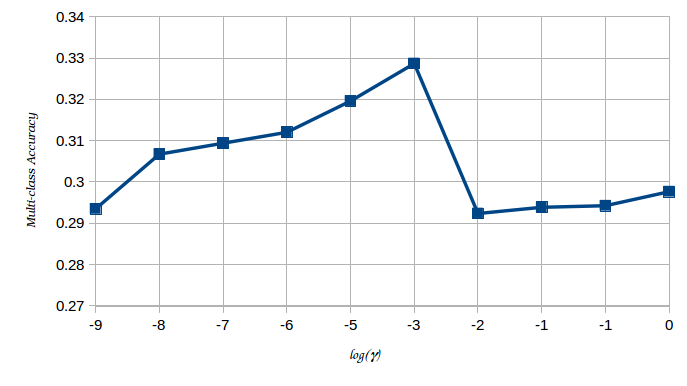
\includegraphics[width=\linewidth]{images/nn_param_apy}
    \caption{aPY}
\end{subfigure}
%
\begin{subfigure}[b]{0.43\linewidth}
    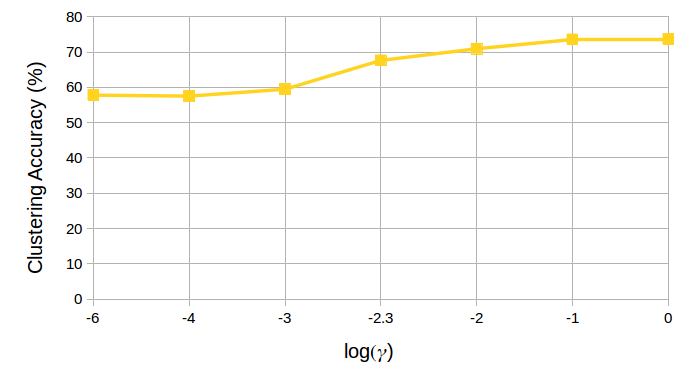
\includegraphics[width=\linewidth]{images/nn_gamma_awa}
    \caption{AwA}
\end{subfigure}
%
\begin{subfigure}[b]{0.43\linewidth}
    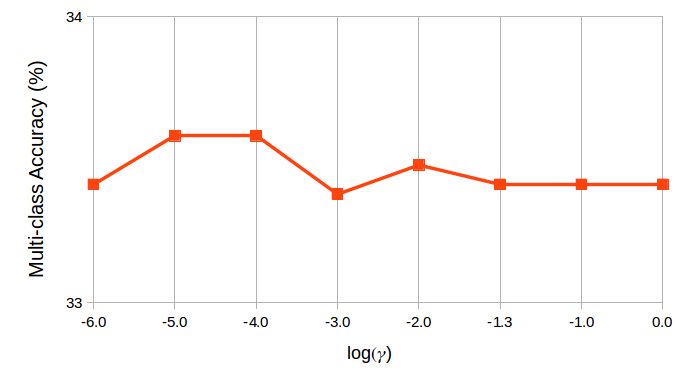
\includegraphics[width=\linewidth]{images/nn_param_birds}
    \caption{CUB-2011}
\end{subfigure}
\begin{subfigure}[b]{0.43\linewidth}
    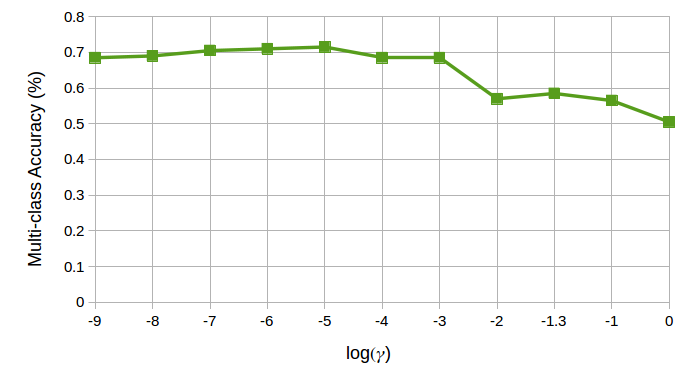
\includegraphics[width=\linewidth]{images/nn_param_sun}
    \caption{SUNA}
\end{subfigure}
\caption[نمودار تحلیل پارامتر شبکه عصبی]{
میزان دقت دسته‌بندی چند دسته‌ای در شبکه چندوظیفه‌ای ارائه شده (نسخه یک لایه) بر حسب $\log_{10}$ پارامتر $\gamma$ در معادله
\eqref{eq:nn_loss}.
}
\label{fig:nn_param}
\end{figure}




\section{بررسی خوشه‌بندی نیمه‌نظارتی}
\begin{table}[ht]
\centering
\caption[بررسی عمل‌کرد خوشه‌بندی نیمه‌نظارتی پیشنهاتی]{
امتیاز معیار دقت (٪) تخصیص خوشه‌ها که با رای‌گیری روی برچسب‌های صحیح به شماره دسته تبدیل شده است؛ بر روی چهار مجموعه داده مورد استفاده در یادگیری بدون نمود نمونه‌ای. نتایج روش پیشنهادی به صورت
\textit{ میانگین $\pm$ انحراف معیار }
برای سه اجرا گزارش شده‌است.}
\vspace*{2mm}
  \label{tab:clustering}
\begin{tabular}{|r|c|c|c|c|}
\hline
روش خوشه‌بندی & AwA & CUB-2011 & aPY & SUNA \\
\hline
k-means                             &  ${65.93 \pm 1.73}$                 & ${34.48 \pm 1.00}$           & ${65.37 \pm 3.73 }$               & ${16.83 \pm 0.76 }$   \\
\hline
خوشه‌بندی نیمه‌نظارتی (بخش \ref{clustering_method})
                      & \textbf{${70.74\pm 0.32}$}  & \textbf{${42.63\pm 0.07}$} & \textbf{${69.93\pm 3.40}$} & \textbf{ ${45.50 \pm 1.32}$} \\
\hline
\end{tabular}
\vspace{2mm}
\end{table}

در این بخش به بررسی عمل‌کرد روش خوشه‌بندی نیمه‌نظارتی ارائه شده در بخش \ref{clustering_method} می‌پردازیم. برای این منظور روش ارائه شده را روی هر مجموعه داده اجرا کرده، خوشه‌های مربوط به دسته‌های دیده‌شده را کنار گذاشته  و هر یک از خوشه‌های دیگر را به یک دسته از دسته‌های آزمون نسبت می‌دهیم. برای این کار در هر خوشه بر اساس برچسب صحیح نمونه‌ها رای‌گیری می‌شود و برچسبی که بیشتر اعضای آن خوشه آن را دارا هستند به کل اعضای خوشه نسبت داده می‌شود. نتیجه با برچسب‌های صحیح مقایسه شده و \gls{mulit-class-accurary} در جدول \ref{tab:clustering} گزارش شده است.
 برای مقایسه عمل‌کرد، آزمایش مشابهی را با روش \lr{k-means} اجرا می‌کنیم. به این صورت که  الگوریتم \lr{k-means} را با $k=n_s + 2n_u$ اجرا کرده و با هر خوشه با رای‌گیری برچسب یکی از دسته‌های دیده نشده را نسبت می‌دهیم. نتایج مربوط به این آزمایش نیز در جدول \ref{tab:clustering} گزارش شده است.

%  در آزمایش‌های فوق پارامترهای $k$ و $\beta$ در رابطه \eqref{eq:my_clustering} توسط قواعد سرانگشتی ارائه شده در بخش \ref{simple_opt} تنظیم شده‌اند. برای روشن شدن میزان تاثیر این پارامترها در عمل‌کرد این روش خوشه‌بندی، دقت حاصل شده در این خوشه‌بندی بر اساس هر کدام از این پارامترها سنجیده شده و نتیجه در تصویر \ref{fig:cluster_params} ارائه شده است.
%  همان‌طور که دیده می‌شود افزایش تعداد خوشه‌ها باعث افزایش دقت خوشه‌بندی  (با تعریف ارائه شده در بالا) شده است. باید به این نکته توجه کرد که این سیر صعودی طبیعی است و الزاما به معنای عمل‌کرد بهتر روش با تعداد خوشه‌های بیشتر نیست. در حقیقت، در حالت حدی بدیهی، وقتی تعداد خوشه‌ها با تعداد نمونه‌ها برابر شود دقت خوشه‌بندی به ۱ خواهد رسید. چرا که در این حالت هر خوشه تنها یک عضو دارد و با رای‌گیری روی برچسب اعضا، تنها رای همان عضو که برچسب صحیح خود است وجود دارد و در نتیجه تمام خوشه‌ها برچسب صحیحی دریافت خواهند کرد. با توجه به این مسئله، تنظیم این پارامتر با استفاده از اعتبارسنجی روی دقت خوشه‌بندی امکان پذیر نیست چرا که جواب بهینه‌ی آن یک حالت بدیهی خواهد بود. در عوض با توجه به استفاده‌ی ما از این روند خوشه‌بندی در دسته‌بندی بدون نمود نمونه‌ای، این پارامتر باید با توجه به تاثیرش بر دقت دسته‌بندی بدون نمود نمونه‌ای تنظیم شود. در این حالت همان‌طور که نتایج بخش \ref{exp:simple} نشان می‌دهد، دقت دسته‌بندی حساسیت کمی به تعداد خوشه‌ها دارد در نتیجه برای کاهش زمان آموزش توسط یک قاعده سرانگشتی تعیین خواهد شد.
%  تاثیر مقدار پارامتر $\beta$ در دقت خوشه‌بندی نیز در  سمت راست تصویر \ref{fig:cluster_params} قابل مشاهده است، علاوه بر این تاثیر این پارامتر روی دقت نهایی دسته‌بندی بدون نمود نمونه‌ای نیز در بخش \ref{exp:simple} مورد بررسی قرار می‌گیرد. در این پژوهش برای ساده نگه داشتن روش با توجه به تاثیر نه چندان محسوس این پارامتر از اعتبار سنجی روی مقدار این پارامتر نیز صرف‌نظر شده است. امکان تعیین مقدار این اعتبار سنجی دقیقا با روند شرح داده شده در بخش \ref{exp:validation} امکان‌پذیر است و تنها بایست مقادیر کاندید به مجموعه جستجو اضافه شود.
%   \begin{figure}[!h]
%   \centering
%   \begin{subfigure}[b]{0.43\linewidth}
%     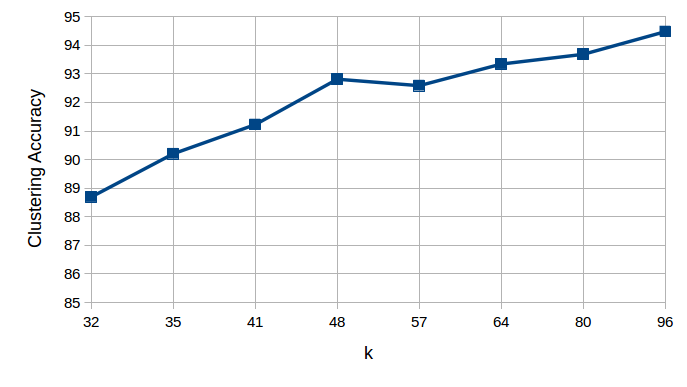
\includegraphics[width=\linewidth]{images/cluster_k_apy}
%     % \caption{\lr{aPY, k}}
%   \end{subfigure}
% %
%   \begin{subfigure}[b]{0.43\linewidth}
%     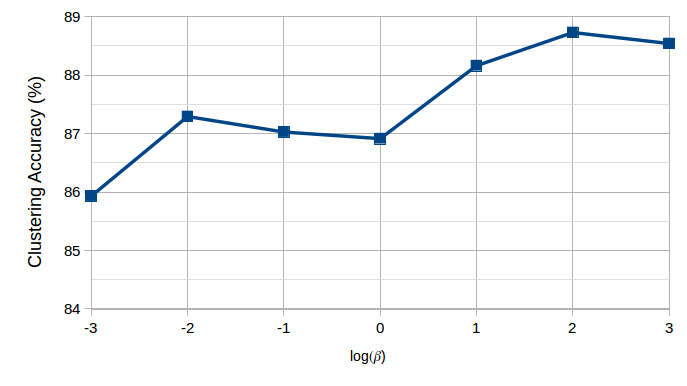
\includegraphics[width=\linewidth]{images/cluster_beta_apy}
%     % \caption{\lr{aPY, $log(\beta)$}}
%   \end{subfigure}
%     \begin{subfigure}[b]{0.43\linewidth}
%     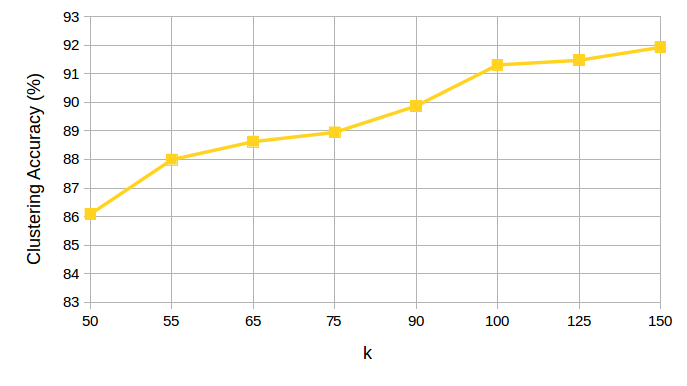
\includegraphics[width=\linewidth]{images/cluster_k}
%     % \caption{\lr{AwA, k}}
%   \end{subfigure}
%     \begin{subfigure}[b]{0.43\linewidth}
%     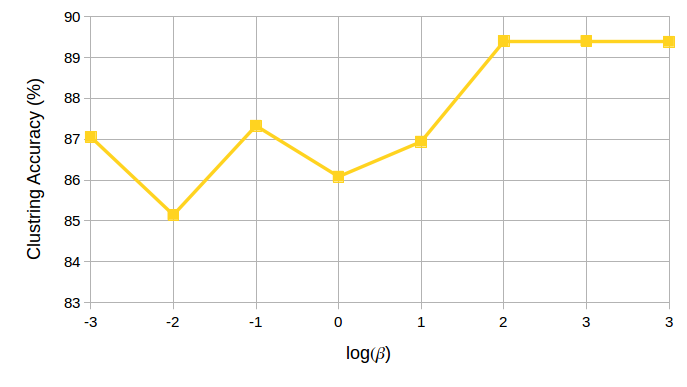
\includegraphics[width=\linewidth]{images/cluster_beta}
%     % \caption{\lr{AwA, $log(\beta)$}}
%   \end{subfigure}
%     \begin{subfigure}[b]{0.43\linewidth}
%     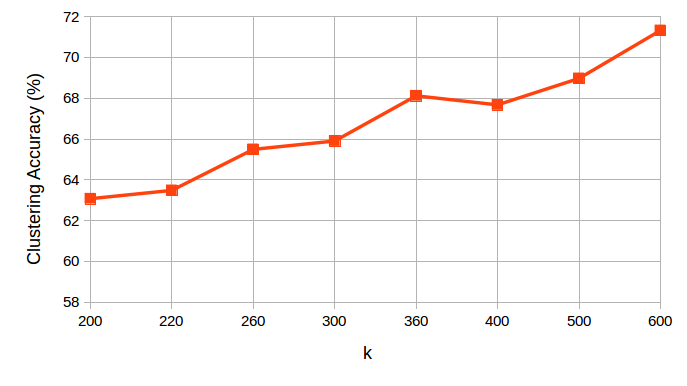
\includegraphics[width=\linewidth]{images/cluster_k_birds}
%     % \caption{\lr{CUB-2011, k}}
%   \end{subfigure}
%     \begin{subfigure}[b]{0.43\linewidth}
%     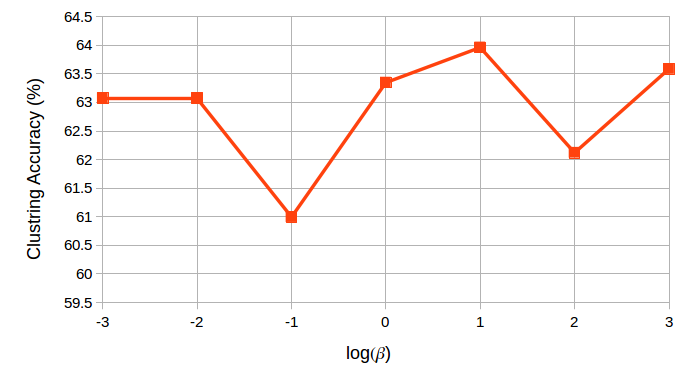
\includegraphics[width=\linewidth]{images/cluster_beta_birds}
%     % \caption{\lr{CUB-2011, $log(\beta)$}}
%   \end{subfigure}
%     \begin{subfigure}[b]{0.43\linewidth}
%     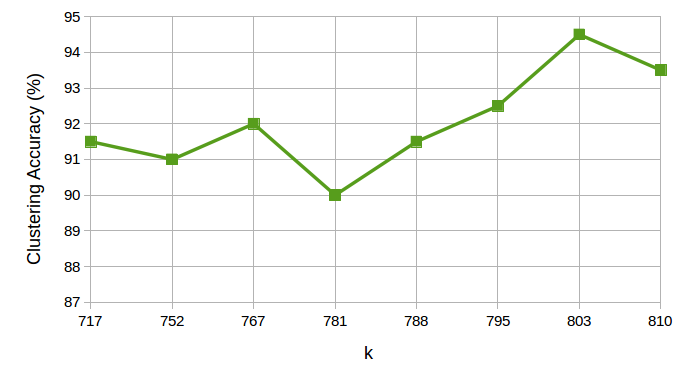
\includegraphics[width=\linewidth]{images/cluster_k_sun}
%   \end{subfigure}
%     \begin{subfigure}[b]{0.43\linewidth}
%     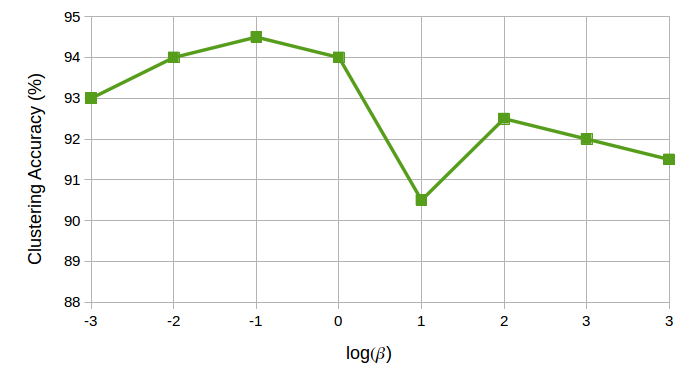
\includegraphics[width=\linewidth]{images/cluster_beta_sun}
%     % \caption{\lr{SUNA $log(\beta)$}}
%   \end{subfigure}
% %
%
%   \caption[
%   تاثیر پارامترهای  روش خوشه‌بندی نیمه‌نظارتی.  ]{
%   تاثیر پارامترهای  روش خوشه‌بندی نیمه‌نظارتی.
% \textbf{سمت چپ}:
%   نتیجه دقت خوشه‌بندی با تغییر تعداد خوشه‌های در نظر گرفته شده.
%  \textbf{سمت راست}:
%  نتیجه دقت  دسته‌بندی چند خوشه‌بندی بر حسب مقادیر پارامتر $\beta$ در رابطه \eqref{eq:my_clustering}.\\
%  برای راحتی مقایسه محور عمودی  همه‌ی نمودارها با بازه‌های یک درصدی تقسیم‌بندی شده‌اند.\\
% سطر اول (آبی‌رنگ): مجموعه دادگان \lr{aPY}. سطر دوم (زرد رنگ): مجموعه دادگان \lr{AwA}. سطر سوم (قرمز رنگ): مجموعه دادگان \lr{CUB-2011}. سطر چهارم (سبز رنگ): مجموعه دادگان \lr{SUNA}.
% %مشاهده توام تاثیر هر دو پارامتر.
% % نتایج نمودارها مربوط به مجموعه دادگان \lr{Animals with Attributes} است.
%  }
%   \label{fig:cluster_params}
%   \end{figure}

\section{نگاشت به هیستوگرام دسته‌های دیده‌شده با شبکه عصبی}
در این بخش به ارائه جزییات پیاده‌سازی و تنظیمات مورد استفاده برای بررسی شبکه‌ی ژرف معرفی شده در بخش \ref{hist} می‌پردازیم.
 در شبکه‌ی عصبی مورد استفاده در این روش، از چهار لایه با اتصالات کامل بعد از لایه‌های پیچشی برگرفته شده از شبکه vgg استفاده شده است. با توجه به این که این شبکه با معیار دسته‌بندی نمونه‌ها در دسته‌های دیده شده آموزش می‌بیند،
 اندازه‌ی لایه‌ی آخر الزاما باید برابر تعداد دسته‌های دیده شده در هر مجموعه دادگان باشد. اندازه سه لایه‌ی قبل از آن برای هر چهار مجموعه‌ دادگان مورد آزمایش برابر ۱۲۰ عدد درنظر گرفته شده است. برای جلوگیری از بیش‌برازش، میان هر دولایه با اتصالات کامل از یک لایه‌ی \gls{dropout} \cite{dropout} استفاده شده؛ احتمال حذف تصادفی در این لایه‌ها برابر $0.4$ در نظر گرفته است.
 تابع فعال‌سازی لایه‌ی پایانی، نسخه‌ای از تابع softmax است که در رابطه \eqref{tsoftmax} معرفی شد. در زمان آموزش این تابع به ازای $T=1$ استفاده می‌شود و در زمان آزمون از $T=15$ استفاده شده است. حساسیت عمل‌کرد شبکه نسبت به مقدار این پارامتر برای مجموعه دادگان \lr{aPascal/aYahoo} در تصویر \ref{hist_param} مورد بررسی قرار گرفته است. مشاهده می‌شود که افزایش مقدار $T$ در ابتدا با هموارتر کردن هیستوگرام حاصل باعث افزایش دقت دسته‌بندی شود اما با ادامه افزایش آن مقادیر هیستوگرام حاصل بسیار به یکدیگیر نزدیک شده و اطلاعات موجود در آن از بین می‌رود در نتیجه دقت دسته‌بندی کاهش می‌یابد.
 \begin{figure}[!t]
\centering
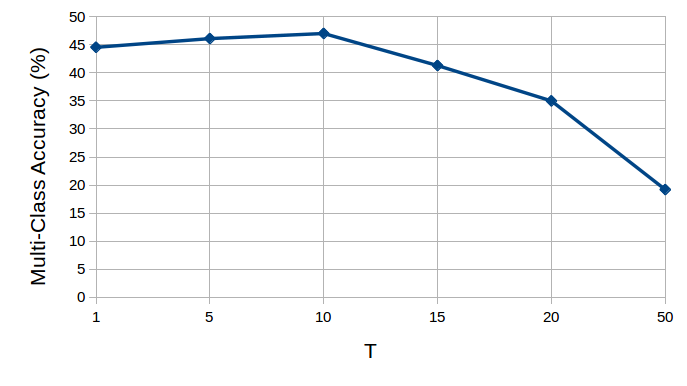
\includegraphics[width=0.75\linewidth]{images/hist_param}
\caption[بررسی تاثیر پارامترهای روش نگاشت به هیستوگرام با شبکه عصبی]{
بررسی میزان دقت دسته‌بندی بر حسب پارامتر $T$ در رابطه \eqref{tsoftmax} برای مجموعه دادگان \lr{aPascal/aYahoo}: افزایش $T$ در ابتدا می‌تواند باعث افزایش دقت شود ولی ادامه افزایش آن باعث نزدیک شدن مقادیر هیستوگرام به یکدیگر و کاهش دقت دسته‌بندی می‌شود.
}
\label{hist_param}
\end{figure}
در سایر لایه‌ها تابع فعال‌سازی ReLU به کار گرفته شده است. آموزش شبکه مطابق با حالت معمول دسته‌بندی با شبکه‌های عصبی  با تابع هزینه آنتروپی متقاطع میان خروجی شبکه و  برچسب صحیح (با کدگذاری یکی‌یک) صورت گرفته است. الگوریتم بهینه‌سازی مورد استفاده برای آموزش شبکه، الگوریتم adadelta \cite{adadelta} است. تعداد تکرارها در آموزش شبکه حداکثر ۸۰ تکرار و \gls{batchsize} برابر ۱۲۸ درنظر گرفته شده است. مدت زمان آموزش شبکه با استفاده از پردازنده گرافیکی
\lr{NVIDIA Geforce Titan Black}
در تمامی آزمایش‌ها کمتر از ۵ دقیقه بوده است.


 نتایج مربوط به این روش در جدول 
 \ref{tab:results} 
با عنوان
\textit{نگاشت به هیستوگرام}
آمده است.  همان‌گونه که مشاهده می‌شود این روش با اینکه از روند ساده و همچنین سریعی بخاطر استفاده از الگوریتم‌های بهینه‌سازی تصادفی برخوردار است، به نتایج بهتری نسبت به روش‌های پیشین دست یافته است و تنها از روش بسیار اخیر ارائه شده در \cite{agnostic} دقت کمتری داشته است. این در حالی‌ست که در سایر روش‌های مبتنی بر هیستوگرام (\cite{sse, agnostic}) از روندهای بهینه‌سازی همراه با محدودیت استفاده می‌شود که بسیار کندتر هستند. برای مثال حداکثر زمان اجرا در \cite{sse} روی چهار مجموعه دادگان مورد بررسی ۳۰ دقیقه اعلام شده است در حالی‌که در آزمایشات انجام شده زمان آموزش شبکه پیشنهادی کمتر از ۵ دقیقه بوده است. همچنین به علت محدودیت‌های روش‌های بهینه‌سازی محدب، این روش‌ها در مجموعه دادگان بزرگ مانند ImageNet قابل استفاده نیستند در حالی‌که روش پیشنهادی دارای قابلیت مقیاس‌پذیری و استفاده در مجموعه دادگان بزرگتر است.
 %
 %
\section{دسته‌بندی با روش خوشه‌بندی و یادگیری نگاشت مجزا } \label{exp:simple}
در این بخش به بررسی عملی روش پیشنهادی برای روش خوشه‌بندی و یادگیری نگاشت مجزای نیمه‌نظارتی می‌پردازیم که  در بخش \ref{simple_method} معرفی شد و مراحل آن در الگوریتم \ref{alg:simple} ذکر شده است. این روش مبتنی بر یک خوشه‌بندی روی داده‌های آزمون بوده و با استفاده از یک نگاشت خطی از فضای توصیف دسته‌ها به فضای تصاویر، مرکز هر خوشه را به یک دسته‌ی دیده نشده منتسب می‌کند. بر اساس تابع مطابقت پیشنهادی (بخش \ref{compatibility_function})، تمام اعضای هر خوشه همان برچسبی که مرکزشان دریافت کرده را دریافت می‌کند.

این روش با استفاده از دو نوع خوشه‌بندی آزمایش شده است. یکی خوشه‌بندی نیمه‌نظارتی پیشنهادی که نتایج این حالت با عنوان
\textit{پیشنهادی (خوشه‌بندی و یادگیری نگاشت مجزا- نیمه‌نظارتی) }
در جدول \ref{tab:results} آمده است.
 برای بررسی تاثیر خوشه‌بندی ارائه شده یک نسخه دیگر از این روش که در آن از خوشه‌بندی \lr{k-means} بجای خوشه‌بندی پیشنهادی استفاده شده است نیز مورد آزمایش قرار گرفته است. نتایج مربوط به این روش با عنوان
\textit{ پیشنهادی (خوشه‌بندی و یادگیری نگاشت مجزا + \lr{k-means} ) }
آمده است.  همان‌گونه که از نتایج مشخص است، استفاده از خوشه‌بندی نیمه‌نظارتی ارائه شده همواره نتایج بهتری نسبت به استفاده از خوشه‌بندی  \lr{k-means} تولید کرده است.

 تاثیر پارامترهای مورد استفاده در این روش در شکل \ref{fig:simple_params} آمده است. همان‌طور که مشاهده می‌شود \gls{hyperparameter} $\eta$ در رابطه
 \eqref{eq:d_answer}
تاثیر قابل توجهی بر دقت دسته‌بندی نهایی دارد، در نتیجه ما مقدار این \gls{hyperparameter} را با استفاده از روند اعتبارسنجی شرح داده شده در بخش \ref{exp:validation} تنظیم کرده‌ایم. از طرف دیگر مشاهده می‌شود تعداد خوشه‌ها در خوشه‌بندی نیمه‌نظارتی ارائه شده تاثیر قابل توجهی بر دقت دسته‌بندی ندارد و تنظیم آن‌ها با قواعد سرانگشتی بیان شده در بخش  \ref{clustering_method} در تمام موارد دقت دسته‌بندی بالایی ایجاد می‌کند.

 \begin{figure}[!h]
   \captionsetup[subfigure]{labelformat=empty, font=footnotesize}
  \centering
  \begin{subfigure}[b]{0.3\linewidth}
    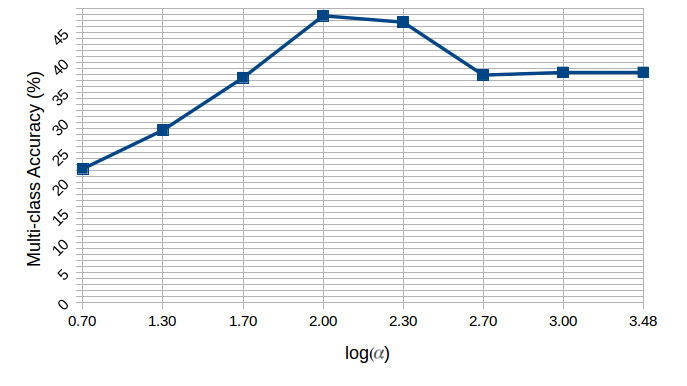
\includegraphics[width=\linewidth]{images/simple_gamma}
  \end{subfigure}
  \begin{subfigure}[b]{0.3\linewidth}
    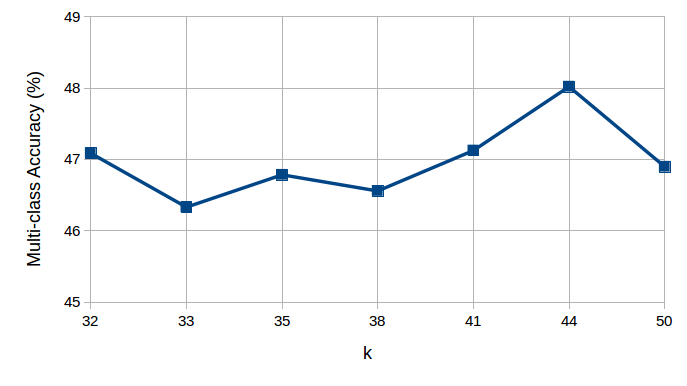
\includegraphics[width=\linewidth]{images/simple_k}
  \end{subfigure}
    \begin{subfigure}[b]{0.3\linewidth}
    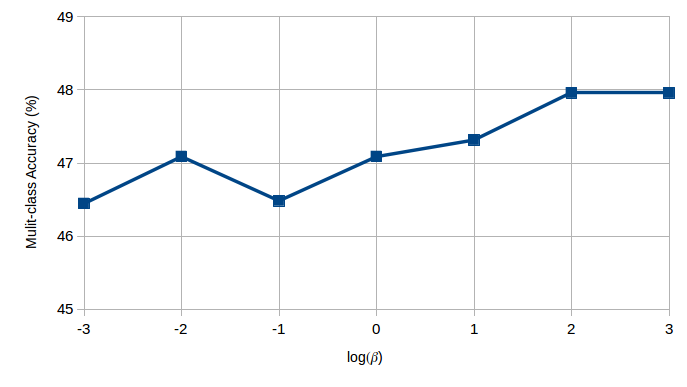
\includegraphics[width=\linewidth]{images/simple_beta}
  \end{subfigure}
  %%%%%%%%%%%%
    \begin{subfigure}[b]{0.3\linewidth}
    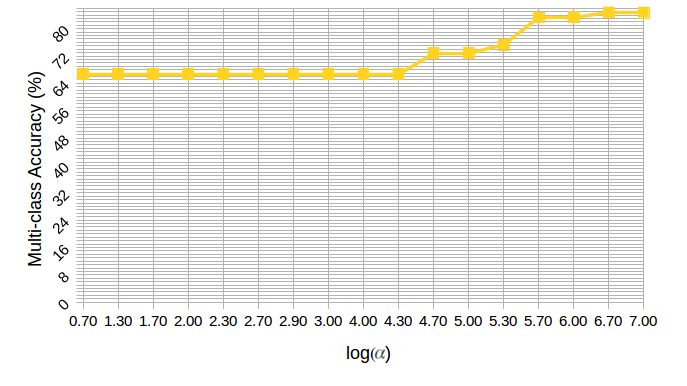
\includegraphics[width=\linewidth]{images/simple_gamma_awa}
  \end{subfigure}
  \begin{subfigure}[b]{0.3\linewidth}
    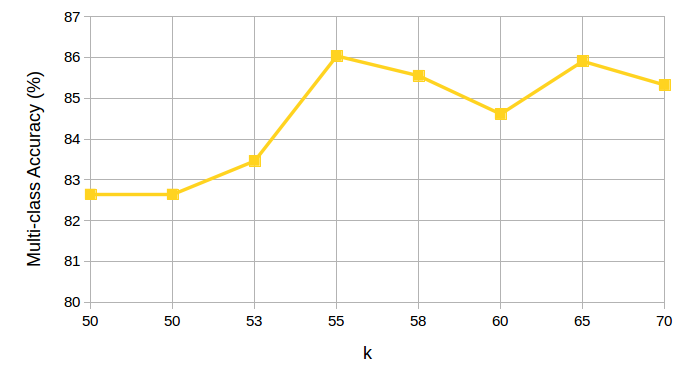
\includegraphics[width=\linewidth]{images/simple_k_awa}
  \end{subfigure}
    \begin{subfigure}[b]{0.3\linewidth}
    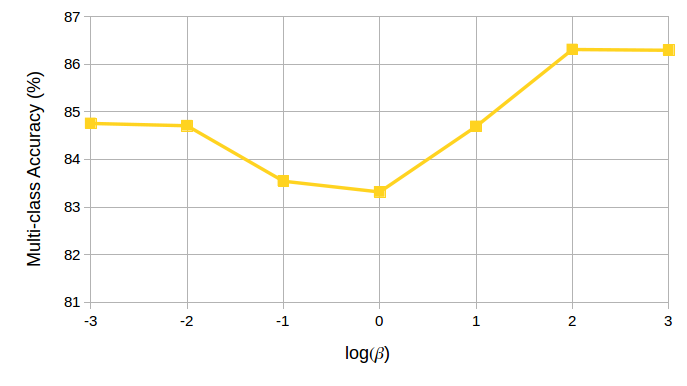
\includegraphics[width=\linewidth]{images/simple_beta_awa}
  \end{subfigure}
  %
    \begin{subfigure}[b]{0.3\linewidth}
    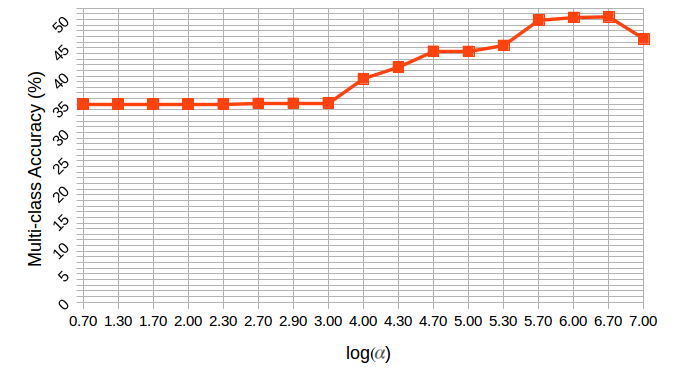
\includegraphics[width=\linewidth]{images/simple_gamma_birds.png}
  \end{subfigure}
  \begin{subfigure}[b]{0.3\linewidth}
    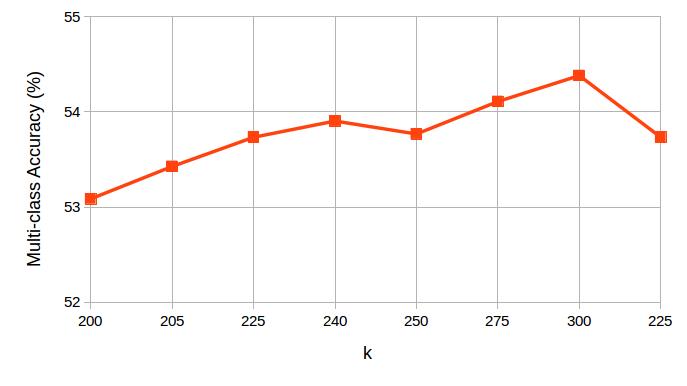
\includegraphics[width=\linewidth]{images/simple_k_birds.png}
  \end{subfigure}
    \begin{subfigure}[b]{0.3\linewidth}
    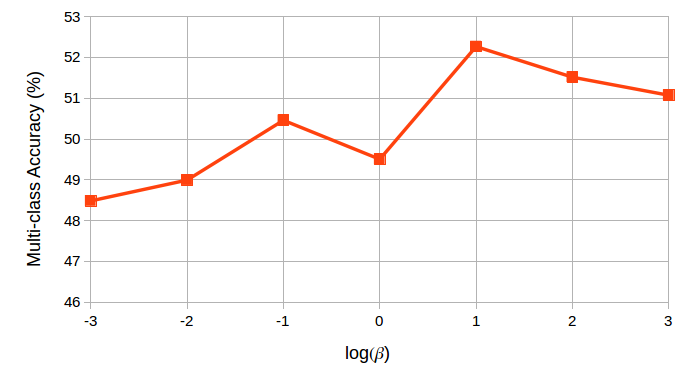
\includegraphics[width=\linewidth]{images/simple_beta_birds.png}
  \end{subfigure}
  %%00000000000000000000000000000
    \begin{subfigure}[b]{0.3\linewidth}
    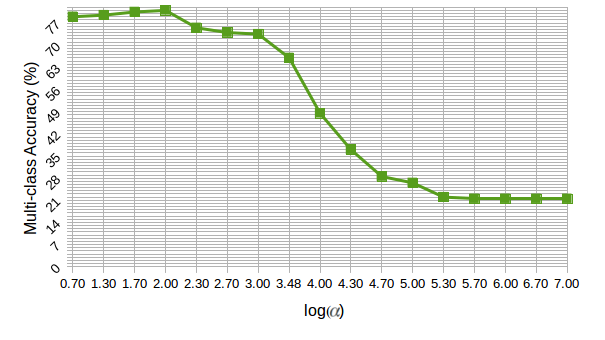
\includegraphics[width=\linewidth]{images/simple_gamma_sun.png}
  \end{subfigure}
  \begin{subfigure}[b]{0.3\linewidth}
    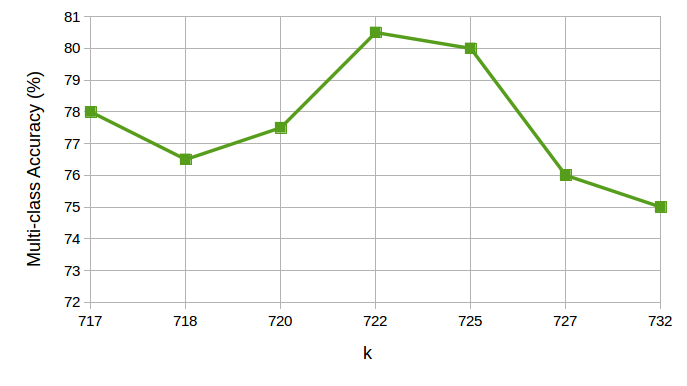
\includegraphics[width=\linewidth]{images/simple_k_sun}
  \end{subfigure}
  \begin{subfigure}[b]{0.3\linewidth}
    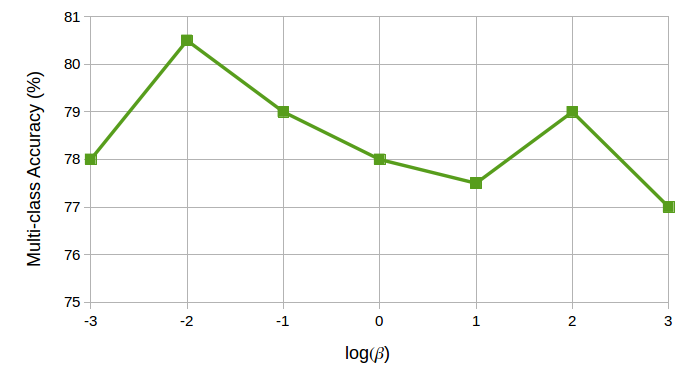
\includegraphics[width=\linewidth]{images/simple_beta_sun}
  \end{subfigure}
  \caption[تحلیل پارامترهای روش دسته‌بندی با خوشه‌بندی نیمه‌نظارتی]{
  تاثیر پارامترهای  روش خوشه‌بندی و یادگیری نگاشت مجزای نیمه‌نظارتی.    \textbf{سمت چپ}: نتیجه دقت دسته‌بندی چند دسته‌ای بدست آمده بر حسب \gls{hyperparameter}  $\alpha$ در رابطه
 \eqref{eq:d_answer}
 که اهمیت جمله منظم‌سازی را نشان می‌دهد. همان‌طور که مشاهده می‌شود، عمل‌کرد روش به این \gls{hyperparameter} حساس است.
 \textbf{وسط }:
 نتیجه دقت  دسته‌بندی چند دسته‌ای بدست آمده بر حسب تعداد خوشه‌ها در خوشه‌بندی نیمه‌نظارتی. با توجه مقیاس این نمودار مشخص می‌شود که دقت حاصل شده حساسیت کمی نسبت به این پارامتر دارد.
  \textbf{سمت راست}:
  نتیجه دقت دسته‌بندی چنددسته‌بای بر حسب پارامتر $\beta$ در خوشه‌بندی نیمه نظارتی (رابطه \eqref{eq:my_clustering}).\\
  برای راحتی مقایسه محور عمودی  همه‌ی نمودارها با بازه‌های یک درصدی تقسیم‌بندی شده‌اند.\\
سطر اول (آبی‌رنگ): مجموعه دادگان \lr{aPY}. سطر دوم (زرد رنگ): مجموعه دادگان \lr{AwA}. سطر سوم (قرمز رنگ): مجموعه دادگان \lr{CUB-2011}. سطر چهارم (سبز رنگ): مجموعه دادگان \lr{SUNA}.
 }
  \label{fig:simple_params}
  \end{figure}




\section{ خوشه‌بندی و یادگیری نگاشت توام}\label{exp:jeac}
\label{exp:cluster}
روش پیشنهادی دوم که در بخش \ref{jeac} ارائه شد به خوشه‌بندی و یادگیری نگاشت توام پرداخته و برچسب نمونه‌های آزمون در آن به طور مستقیم در جریان آموزش بدست می‌آید.
تنظمیات آزمایش برای روش خوشه‌بندی و نگاشت توام مانند حالت قبل سه بار اجرا و گزارش نتایج به صورت \textit{ میانگین $\pm$ انحراف معیار } است. این روش با دو نوع  مقداردهی اولیه آزمایش شده است. روش اول، مقداردهی $R$ که با استفاده از الگوریتم
\ref{alg:simple}
انجام می‌شود؛ نتایج مربوط به این حالت در جدول  \ref{tab:results} با عنوان
\textit{ پیشنهادی (توام، مقداردهی $R$)}
آمده‌اند. روش دوم مقداردهی اولیه ، شروع بهینه‌سازی تناوبی در الگوریتم
\ref{alg:jeac}
 با مقداردهی $D$ است که توسط رابطه
\eqref{eq:d_answer}
صورت گرفته است. نتایج مربوط به این حالت با عنوان
\textit{پیشنهادی (توام، مقداردهی $D$)}
آمده‌اند. مقایسه نتایج مربوط به این دو نحوه‌ی مقداردهی اولیه نشان می‌دهد که استفاده از روش پیشنهادی الگوریتم \ref{alg:simple}  برای رسیدن به دقت بالا ضروری است، چرا که مشاهده می‌شود که استفاده از مقداردهی اولیه برای $R$ به صورت بیان شده در الگوریتم \ref{alg:jeac} به طور متوسط $6.8$٪ دقت بالاتری در دسته‌بندی نسبت به مقداردهی $D$  با رابطه \eqref{eq:d_answer} دارد. دلیل این موضوع همان‌طور که در بخش \ref{jeac} بیان شد استفاده از اطلاعات بدون نظارت نمونه‌های آزمون در بدست آوردن مقدار اولیه برای $R$ است در حالیکه در مقداردهی اولیه $D$ تنها نمونه‌های آموزش دخالت دارند.

به علت حساسیت نتایج این روش به پارامترهای آن  (مقادیر  $\lambda$ و $\eta$ در رابطه \eqref{eq:joint})، مقادیر آن‌ها توسط روند اعتبارسنجی شرح داده شده در بخش
\ref{exp:validation}
تنظیم می‌شود.
%میزان تاثیر مقادیر این دو پارامتر در نتیجه روش در تصویر \ref{fig:jeac_params} نشان داده شده است. در نمودارهای ارائه شده معیار دقت دسته‌بندی چنددسته‌ای بر حسب مقادیر این دو پارامتر ترسیم شده‌اند.
%  \begin{figure}[!h]
%    \captionsetup[subfigure]{labelformat=empty, font=footnotesize}
%   \centering
%   \begin{subfigure}[b]{0.43\linewidth}
%     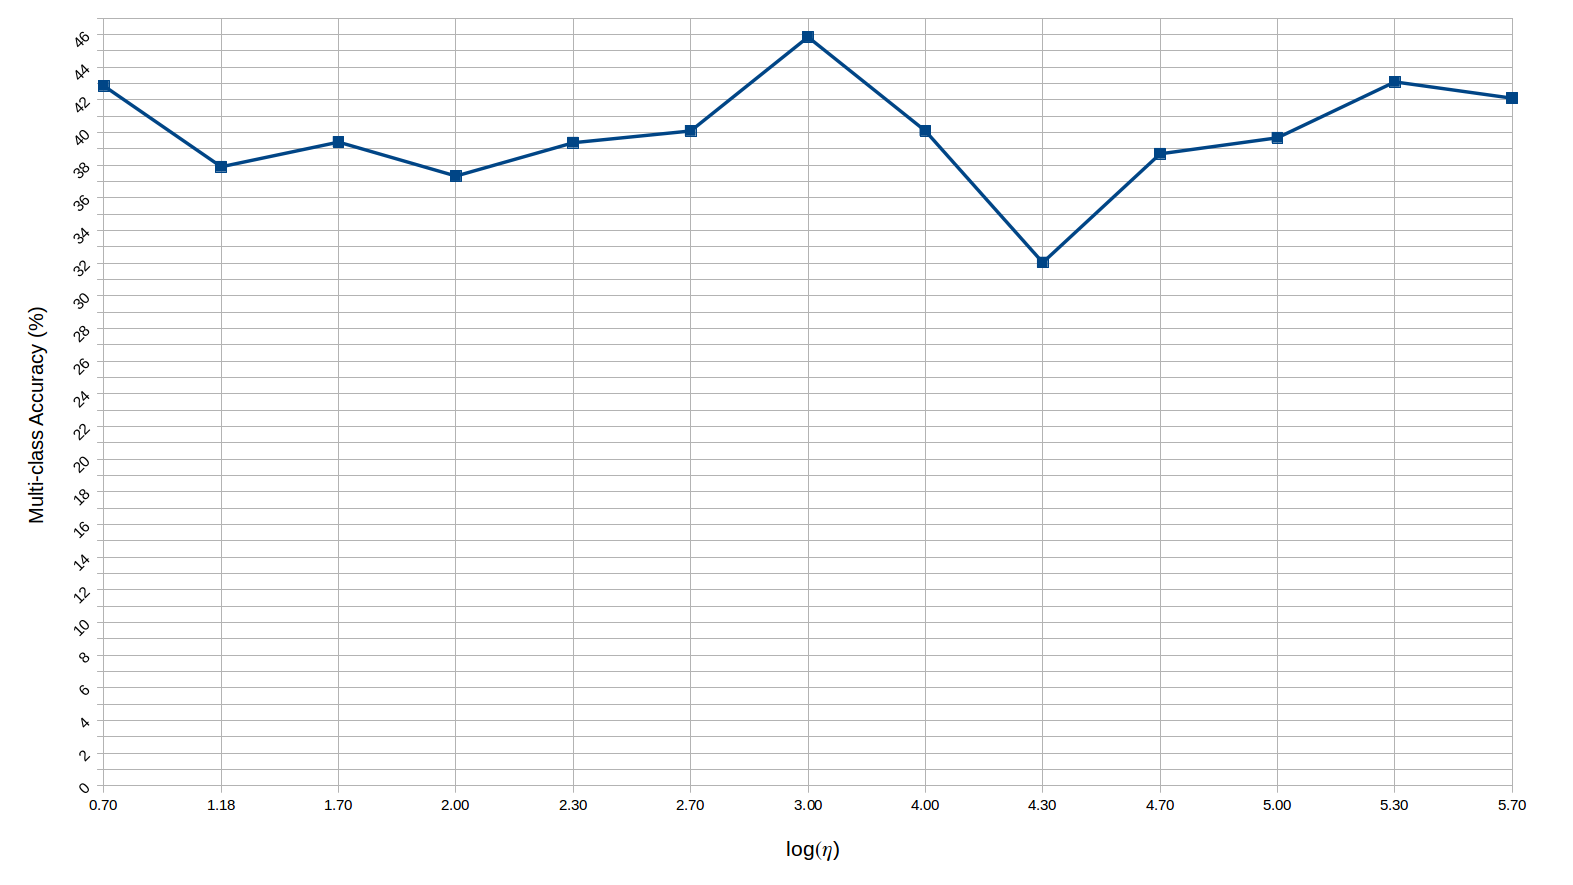
\includegraphics[width=\linewidth]{images/jeac_gamma}
%   \end{subfigure}
%   \begin{subfigure}[b]{0.43\linewidth}
%     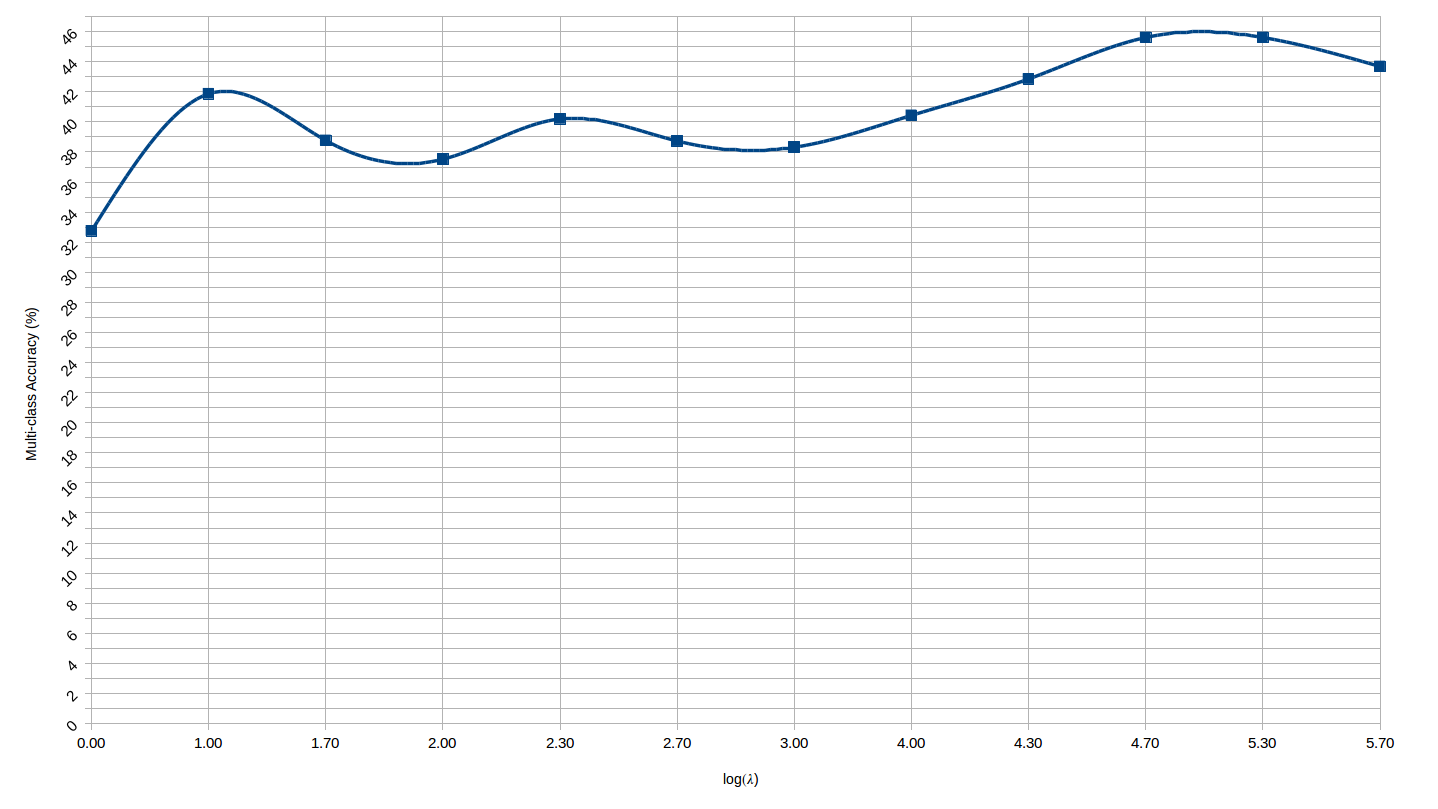
\includegraphics[width=\linewidth]{images/jeac_lambda}
%   \end{subfigure}
%   %%%%%%%%%%%%
%     \begin{subfigure}[b]{0.43\linewidth}
%     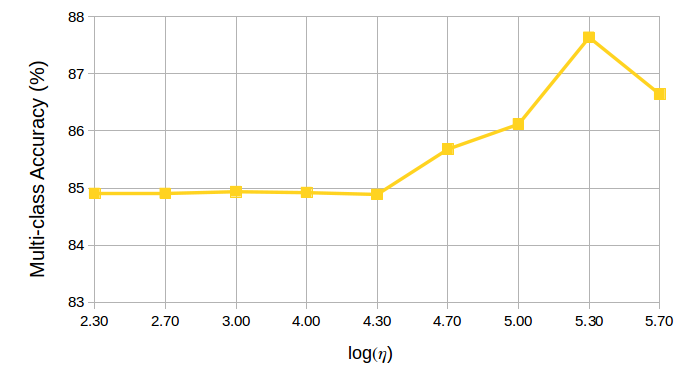
\includegraphics[width=\linewidth]{images/jeac_gamma_awa}
%   \end{subfigure}
%     \begin{subfigure}[b]{0.43\linewidth}
%     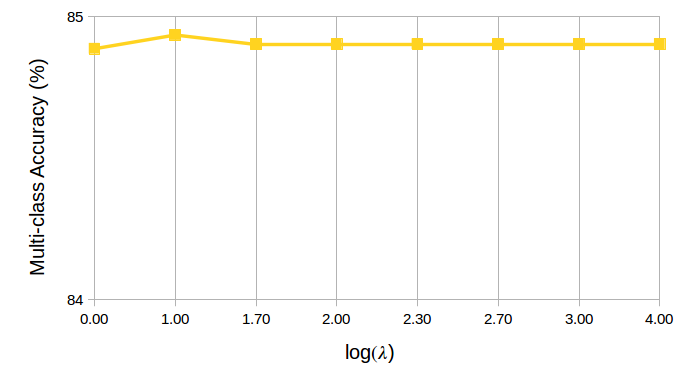
\includegraphics[width=\linewidth]{images/jeac_lambda_awa}
%   \end{subfigure}
%   %
%     \begin{subfigure}[b]{0.43\linewidth}
%     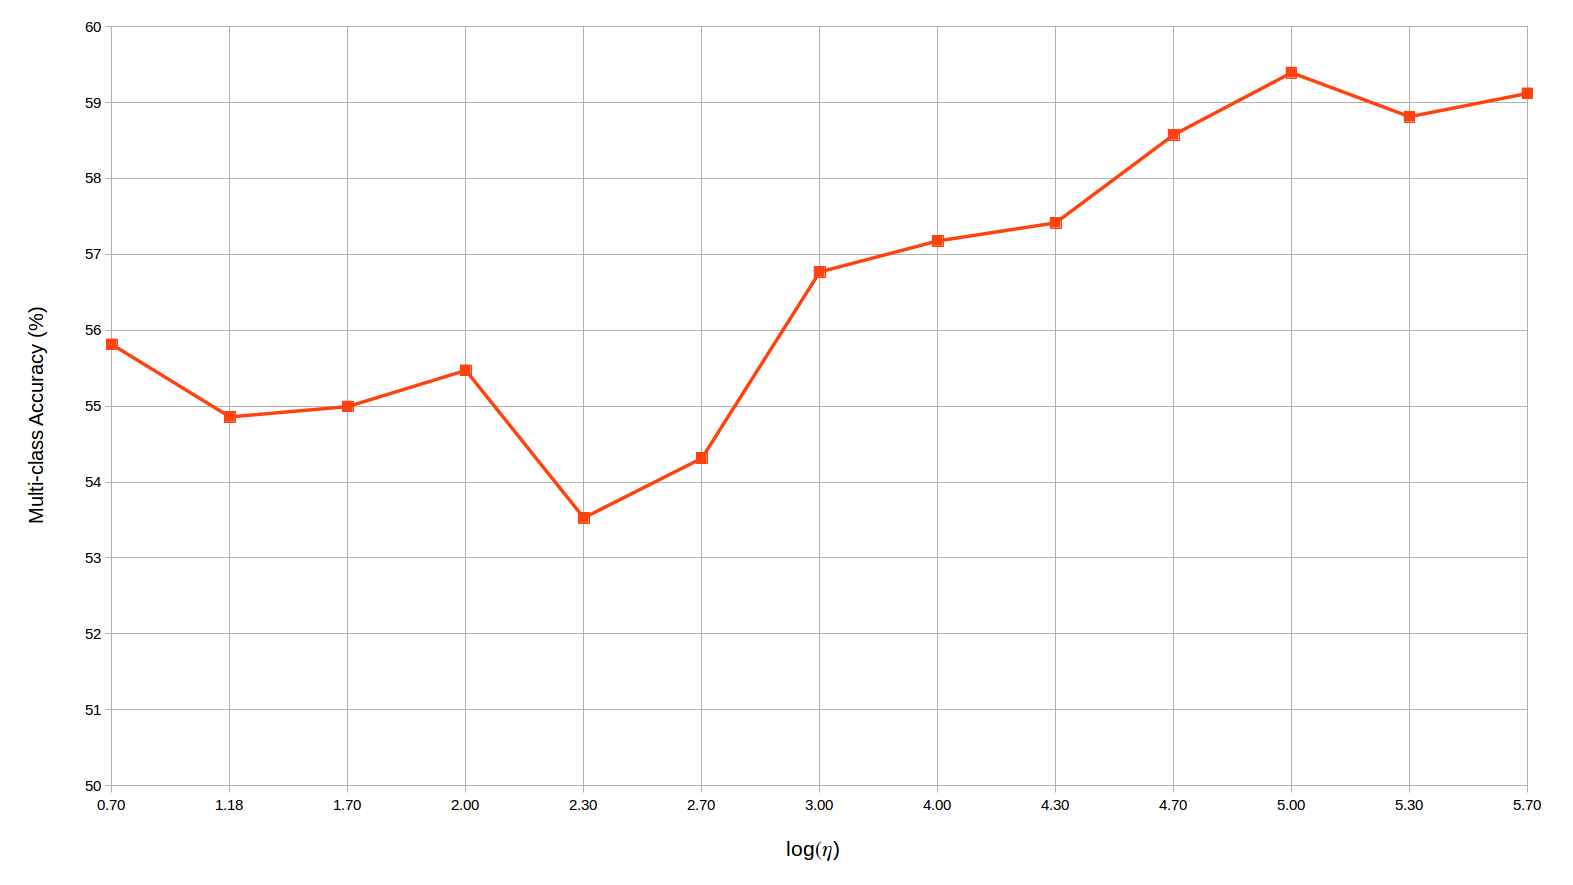
\includegraphics[width=\linewidth]{images/jeac_gamma_birds.png}
%   \end{subfigure}
% \begin{subfigure}[b]{0.43\linewidth}
%     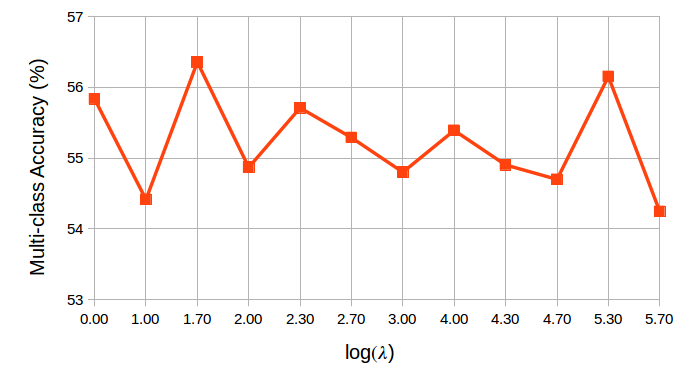
\includegraphics[width=\linewidth]{images/jeac_lambda_birds.png}
%   \end{subfigure}
%   %%00000000000000000000000000000
%     \begin{subfigure}[b]{0.43\linewidth}
%     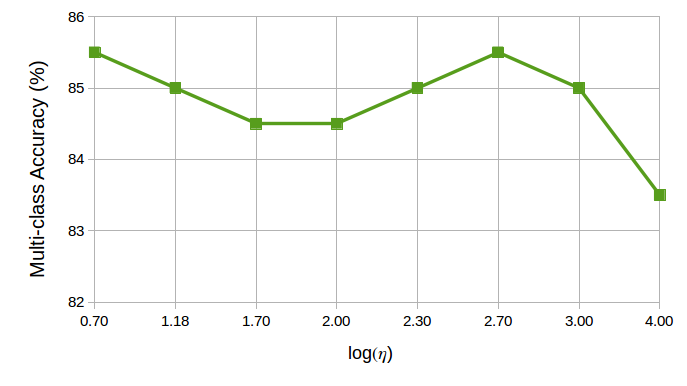
\includegraphics[width=\linewidth]{images/jeac_gamma_sun.png}
%   \end{subfigure}
%   \begin{subfigure}[b]{0.43\linewidth}
%     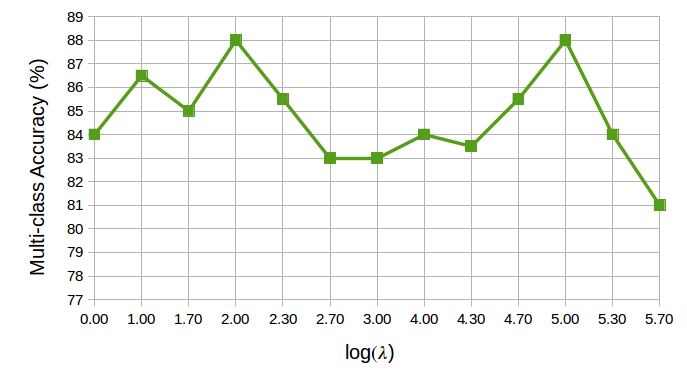
\includegraphics[width=\linewidth]{images/jeac_lambda_sun}
%   \end{subfigure}
%   \caption[تحلیل پارامترهای روش یادگیری نگاشت و خوشه‌بندی توام]{
%   تاثیر پارامترهای  روش یادگیری نگاشت و خوشه‌بندی نیمه‌نظارتی برای مجموعه دادگان مختلف.
% \textbf{سمت چپ:}
%    نتیجه دقت دسته‌بندی چند دسته‌ای بدست آمده بر حسب \gls{hyperparameter}  $\nu$ در رابطه
% \eqref{eq:joint}
%  که اهمیت جمله منظم‌سازی را نشان می‌دهد.
%  % همان‌طور که مشاهده می‌شود، عمل‌کرد روش به این \gls{hyperparameter} حساس است.
%  \textbf{سمت راست}:
%  نتیجه دقت  دسته‌بندی چند دسته‌ای بدست آمده بر حسب مقادیر پارامتر $\lambda$ در رابطه \eqref{eq:joint}
% برای راحتی مقایسه محور عمودی  همه‌ی نمودارها با بازه‌های یک درصدی تقسیم‌بندی شده‌اند.\\
% سطر اول (آبی‌رنگ): مجموعه دادگان \lr{aPY}. سطر دوم (زرد رنگ): مجموعه دادگان \lr{AwA}. سطر سوم (قرمز رنگ): مجموعه دادگان \lr{CUB-2011}. سطر چهارم (سبز رنگ): مجموعه دادگان \lr{SUNA}.
%  }
%   \label{fig:jeac_params}
%   \end{figure}

\subsection{روش‌های مورد مقایسه}\label{exp:other_methods}
 در جدول 
  \ref{tab:results}
 روش‌های پیشنهادی در بخش‌های \ref{hist} و  \ref{simple_method} و \ref{jeac}   با مطرح‌ترین روش‌های اخیر در حوزه یادگیری بدون نمود نمونه‌ای مقایسه شده‌اند.
سایر روش‌هایی که برای مقایسه آورده شده‌اند، روش‌هایی هستند که بالاترین دقت‌های دسته‌بندی را در دسته‌بندی بدون نمود نمونه‌ای دارا هستند و بجز یک مورد تمامی آن‌ها در سال‌های ۲۰۱۵ و ۲۰۱۶ ارائه شده‌اند.
روش‌های ارائه شده در
\cite{li15max, semi15, Kodirov2015}
از این جهت که \textit{نیمه‌نظارتی} هستند، یعنی از  نمونه‌های آزمون نیز در زمان آموزش استفاده می‌کنند، با روش‌های ما بیشترین نزدیکی را دارند. البته در
\cite{li15max, semi15}
از ویژگی‌های کم‌عمق برای تصاویر استفاده شده است که توانایی جداسازی دسته‌ها در آن بسیار پایین‌تر از ویژگی‌های بدست آمده از شبکه‌های عصبی ژرف است که در روش‌های پیشنهادی ما مورد استفاده قرار گرفته است. روش‌های
\cite{Akata2015, Xian2016}
با استفاده از توابع هزینه‌ی بیشترین حاشیه سعی در یادگیری نگاشت از هر دو فضای تصاویر و توصیف دسته‌ها به فضای مشترک دارند. این روش‌ها از ویژگی‌های شبکه‌ی ژرف
\lr{GoogleNet}
 \cite{googlenet}
 برای استخراج ویژگی استفاده می‌کنند. ابعاد ویژگی‌های بدست آمده ۱۰۲۴ است که بعد کمتری نسبت به ویژگی‌های ۴۰۹۶-بعدی استخراج شده از شبکه ۱۹ لایه‌ی vgg دارد و توانایی جداسازی دسته‌ها در آن پایین‌تر است. همان‌طور که مشاهده می‌شود استفاده از این ویژگی‌های با بعد بیشتر عمل‌کرد روش ارائه شده در \cite{Akata2015} را بهبود داده است.

 روش‌هایی که بهترین نتایج را در میان روش‌های رقیب کسب کرده‌اند، روش ارائه شده در \cite{sse} و تعمیم آن در \cite{agnostic}  هستند. هرچند این روش‌ها نیمه‌نظارتی نیستند و تنها از نمونه‌های آموزش برای یادگیری نمایش تصاویر و توصیف دسته‌ها در یک فضای مشترک، که فضای هیستوگرام دسته‌های دیده شده است استفاده می‌کنند، نتایج بهتری نسبت به روش‌های نیمه‌نظارتی پیشین در \cite{li15max, semi15, Kodirov2015} کسب کرده‌اند. این مسئله می‌توان نشان‌گر یک مسیر مناسب در ترکیب روش پیشنهادی در این پژوهش با فضای مشترک مورد استفاده در آن روش‌ها برای کارهای آتی باشد.

\begin{table}[ht]
\centering
\caption [مقایسه دقت دسته‌بندی]{
مقایسه دقت دسته‌بندی چنددسته‌ای روش پیشنهادی با سایر روش‌ها. نتایج بر اساس نوع ویژگی مورد استفاده برای تصاویر دسته‌بندی شده‌اند. جدول شامل دقت دسته‌بندی چنددسته‌ای به صورت
(میانگین $\pm$ انحراف معیار) است. نتایج سایر روش‌ها از مقالاتی که روش در آن‌ها ارائه شده نقل شده و آزمایش‌ها توسط ما تکرار نشده است.
خانه‌هایی که با خط تیره مشخص شده‌اند به معنای عدم ارائه نتایج برای آن مجموعه دادگان در مقاله اصلی روش مورد مقایسه هستند.
 نتایج روش‌های پیشنهادی حاصل سه اجرا هستند.
}
\vspace{4mm}
 \label{tab:results}
 {\scriptsize
\begin{tabular}{|r|r|c|c|c|c|}
\hline
ویژگی تصاویر & روش  & AwA & CUB-2011 & aPY & SUN \\
\hline
{کم‌عمق}
& \lr{Li and Guo } \cite{li15max}                 &  $38.2 \pm 2.3$   &    -             &  -                       & $18.9 \pm 2.5$ \\
& \lr{Li \textit{et al.}}~\cite{semi15}                    &  $40.05\pm 2.25$ &       -          &   $24.71 \pm 3.19$       & -    \\
& \lr{Jayaraman and Grauman}  \cite{jayaraman14}  & $43.01 \pm 0.07$ &       -          & $26.02 \pm 0.05$        & $56.18 \pm 0.27$ \\
\hline
{GoogleNet}
& \lr{Akata \textit{et al.}}~\cite{Akata2015}              & $66.7$          & $50.1$            &         -                & -\\
%& \lr{Changpinyo \textit{et al.}}~\cite{Synthesized}       & $72.9$           & $54.5$            &                         & $62.7$ \\
& \lr{Xian \textit{et al.}}~\cite{Xian2016}                & $71.9$            & $45.5$            &        -                 & -\\
\hline
{VGG-19}
&\lr{ Khodirov \textit{et al.}} \cite{Kodirov2015}
                                            & $73.2$            &  $39.5$           & $26.5$                    &  -\\
& \lr{Akata \textit{et al.}}~\cite{Akata2015}              & $61.9$            &  $50.1$           &                 -        & -\\
& \lr{Zhang and Saligrama}  \cite{sse}            &  $76.33 \pm 0.53$ & $30.41 \pm 0.20$ &   $46.23 \pm 0.53$      & $82.50 \pm 1.32$    \\
& \lr{Zhang and Saligrama} \cite{agnostic}       &  $80.46 \pm 0.53$ & $42.11 \pm 0.55$ &   \textbf{$50.35 \pm 2.97$}      & $83.83 \pm 0.29$    \\
&  پیشنهادی (نگاشت به هیستوگرام)
                          & $76.50 \pm 1.02$               & $33.29 \pm 0.21$              & $47.46 \pm 0.31$              & $79.88 \pm 0.42$ \\
&  پیشنهادی (خوشه‌بندی و یادگیری نگاشت مجزا + \lr{kmeans})
                          & $86.34 \pm 0.13$               & $52.48 \pm 0.60$              & $48.03 \pm 1.56$              & $75.75 \pm 1.06$ \\
& پیشنهادی (خوشه‌بندی و یادگیری نگاشت مجزا - نیمه‌نظارتی)
                        & $86.38 \pm 0.56$              & $ 53.10\pm 0.43 $             & $48.52 \pm 0.29$              &$ 80.66 \pm 0.76$ \\
& پیشنهادی (توام، مقداردهی $D$)
                     & $83.03$                        & $57.55$                       & $42.62$          & $72.50$\\
& پشنهادی (توام، مقداردهی $R$)
                     & \textbf{\em $88.64 \pm 0.04$}  & \textbf{\em $58.80 \pm 0.64$} & $49.77 \pm 2.02$ & \textbf{\em $86.16 \pm 0.57$} \\
\hline
\end{tabular}
}
\end{table}

\section{تحلیل نتایج}\label{exp:discussion}
با توجه به جدول \ref{tab:results} روش پیشنهادی یادگیری توام نگاشت و خوشه‌بندی هنگام مقداردهی اولیه مقادیر $R$ مجموعا به بهترین نتایج دست‌یافته است. این روش روی سه مجموعه داد‌ه‌گان از چهار مجموعه که روش‌ها با آن محک زده شده‌اند نتایج بهتری نسبت به سایر روش‌ها دارد و عمل‌کرد پیشگام در حوزه یادگیری بدون نمود نمونه‌ای را ارتقاء داده است. روی مجموعه داده‌گان \lr{aPascal/aYahoo} روش ارائه شده در
\cite{agnostic}
نتایج بهتری کسب کرده است. دلیل این موضوع می‌تواند شباهت بسیار زیاد میان امضای دسته‌ها در این مجموعه دادگان و عدم ایجاد جداسازی بالا میان دسته‌ها توسط این بردارهای توصیف باشد. در روش پیشنهادی یادگیری نگاشت و خوشه‌بندی توام، با توجه به نزدیکی زیاد این بردارهای توصیف، نگاشت آن‌ها در فضای ویژگی تصاویر نیز به یکدیگر نزدیک خواهد بود و جداسازی مناسبی میان نمونه‌های دسته‌های مختلف صورت
نمی‌پذیرد؛ ولی در روش ارائه شده در \cite{agnostic} همان‌گونه که در فصل دوم مرور شد، بردارهای توصیف ورودی
مستقیماً به کار گرفته نمی‌شوند، بلکه از آن‌ها برای بدست آوردن نمایش دیگری برای دسته‌ها  به صورت هیستوگرامی از دسته‌های دیده شده، استفاده می‌شود. وجود این گام می‌تواند مشکل نزدیکی و شباهت زیاد میان امضای دسته‌ها را از بین ببرد. هم‌چنین همان‌طور که در بخش \ref{jeac_opt} بیان شد، مقداردهی اولیه مقادیر $R$ با استفاده از روش خوشه‌بندی و تابع مطابقت پیشنهادی عمل‌کرد بهتری نسبت به مقداردهی اولیه $D$ دارد. از این جدول هم‌چنین کارایی روش خوشه‌بندی نیمه‌نظارتی پیشنهادی نسبت به الگوریتم \lr{k-means} در مسئله یادگیری بدون برد مشخص می‌شود، چرا که در همه‌ی موارد هنگام استفاده از روش خوشه‌بندی نیمه‌نظارتی پیشنهادی در مقایسه با  الگوریتم \lr{k-means} دقت بالاتری در دسته‌بندی حاصل شده است. هر دو حالت این روش ساده که از یک نگاشت خطی و بخش تاثیرگذارتر تابع مطابقت پیشنهادی تشکیل شده‌اند، روی نیمی از چهار مجموعه‌داده‌گان مورد بررسی عمل‌کرد بهتری نسبت به همه‌ی روش‌های پیشین داشته‌اند که نشان‌دهنده کارایی تابع مطابقت پیشنهادی است.

برای تحلیل کارایی روش‌های خوشه‌بندی و یادگیری نگاشت مجزا و توام و تاثیر قسمت‌های مختلف آن‌ها، 
نتایج به کارگیری هر قسمت از آن‌ها،
  روی یک مجموعه داده واقعی، در شکل
\ref{fig:discussion}
 نشان داده شده است. نتایج مربوط به اجرای روش روی تمام مجموعه دادگان AwA است، ولی برای این که تغییرات در شکل قابل دنبال کردن باشند تنها چهار دسته در  تصویر نشان داده شده‌اند که دو دسته از آن‌ها دسته‌های دیده شده و دو دسته از دسته‌های دیده نشده هستند. در تصویر
\ref{fig:null}
دسته‌های دیده شده به صورت رنگی و دسته‌های دیده نشده با رنگ سیاه مشخص شده‌اند. در تصویر
\ref{fig:truth}
برچسب‌های صحیح برای دسته‌های دیده نشده نیز با رنگ مشخص شده است. در تصویر
\ref{fig:knn}
توصیف دسته‌ها با استفاده از نگاشت $D$ از رابطه \eqref{eq:d_answer} به فضای تصاویر برده شده (نماد ستاره) و سپس نمونه‌های آزمون با استفاده از دسته‌بند نزدیکترین همسایه دسته‌بندی شده‌اند، نمونه‌هایی که رنگ قرمز دارند به دسته‌ای غیر از چهار دسته‌ی موجود در تصویر دسته‌بندی شده‌اند. تصویر
\ref{fig:kmeans}
حاصل دسته‌بندی به شیوه‌ی روش خوشه‌بندی و یادگیری نگاشت مجزای نیمه‌نظارتی ارائه شده در بخش \ref{simple_method} است که در آن از خوشه‌بندی \lr{k-means} و تابع مطابقت پیشنهادی استفاده شده است. تصویر
\ref{fig:clustering}
مشابه حالت قبل است با این تفاوت که در آن از خوشه‌بندی نیمه‌نظارتی پیشنهادی به‌جای \lr{k-means} استفاده شده است. در تصویر
\ref{fig:jeac}
دسته‌بندی و یادگیری نمایش توصیف دسته‌ها در فضای تصاویر (ستاره‌ها) به صورت توام با روش پیشنهادی بخش \ref{jeac} صورت گرفته است.
همان‌طور که در تصاویر
\ref{fig:kmeans} و \ref{fig:clustering}
مشخص است، استفاده از  تابع مطابقت معرفی شده در بخش \ref{compatibility_function} برای دسته‌بندی بسیار موفق‌تر از دسته‌بند نزدیک‌ترین همسایه عمل می‌کند و اطلاعات غیر نظارتی موجود در نمونه‌های آزمون دقت  دسته‌بندی را بهبود می‌دهد. هم‌چنین برتری روش خوشه‌بندی پیشنهادی در تصویر \ref{fig:clustering} قابل مشاهده است. در تصاویر \ref{fig:knn} تا \ref{fig:clustering} که از نگاشت  \eqref{eq:d_answer} برای تصویر کردن توصیف‌ها در فضای تصاویر استفاده شده است، مشکل جابجایی دامنه کاملا قابل رویت است، یعنی برای دسته‌های دیده شده توصیف‌ها به صورت مناسبی در مرکز نمونه‌های آن دسته نگاشته شده‌اند حال آن که برای دسته‌های دیده نشده جابجایی وجود دارد و حاصل نگاشت توصیف این دسته‌ها،  از نمونه‌هایشان فاصله گرفته‌است؛ اما در تصویر
\ref{fig:jeac}
که از روش خوشه‌بندی و یادگیری نگاشت توام استفاده شده است، این مشکل برطرف شده و توصیف‌های دسته‌های دیده نشده نیز مانند دسته‌های دیده شده به مرکز نمونه‌های مربوط به خودشان نگاشته شده‌است.

\begin{figure}[t]
  \centering
  \begin{subfigure}[b]{0.38\linewidth}
    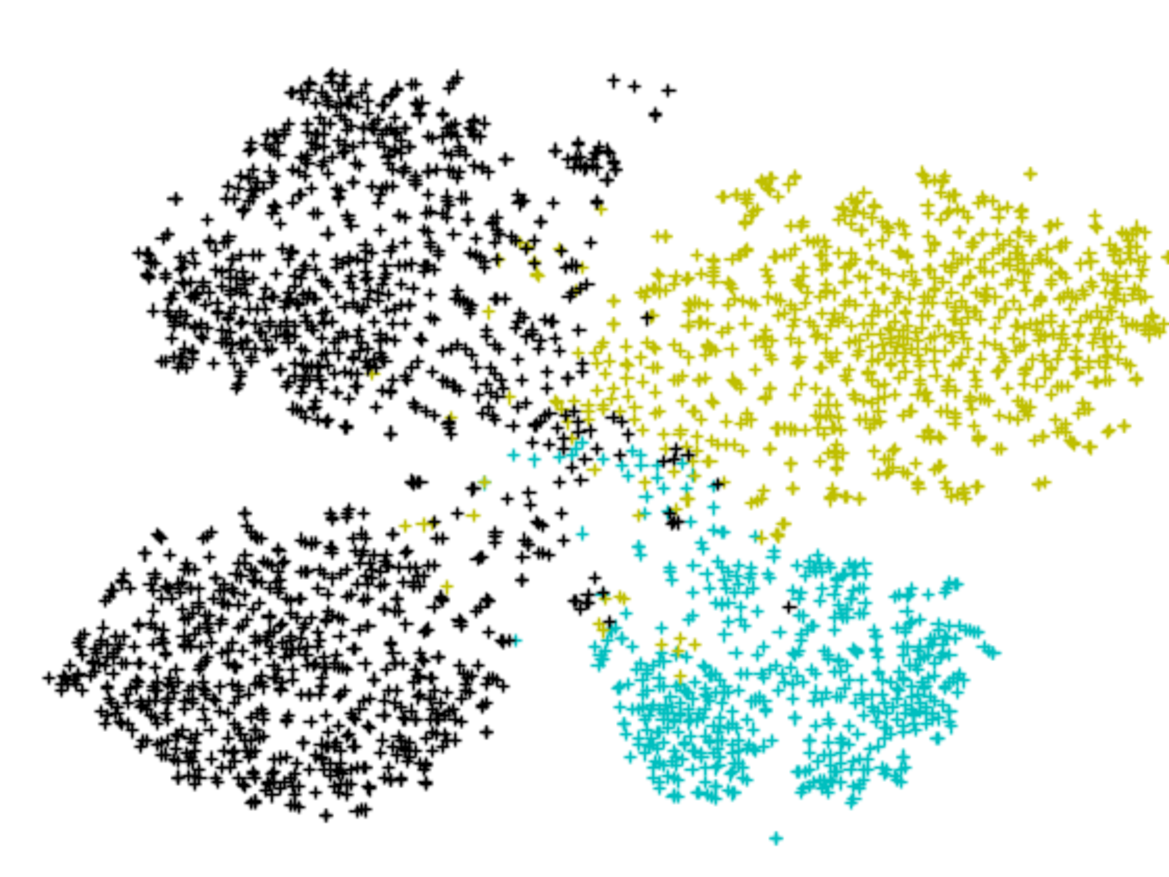
\includegraphics[width=\linewidth]{images/none}
    \caption{}
    \label{fig:null}
  \end{subfigure}
%
  \begin{subfigure}[b]{0.38\linewidth}
    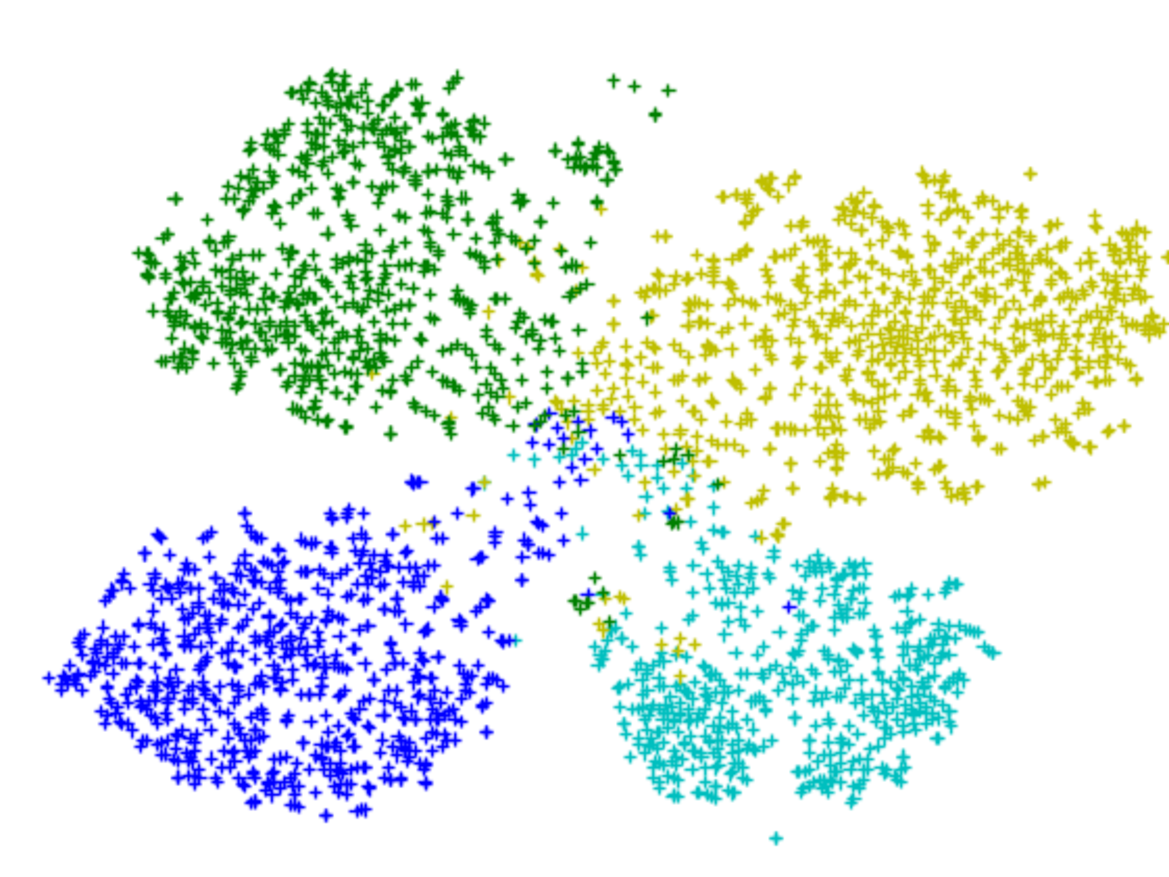
\includegraphics[width=\linewidth]{images/truth}
    \caption{}
% \caption{Points colored according to their ground truth labels}
    \label{fig:truth}
  \end{subfigure}
%
  \begin{subfigure}[b]{0.38\linewidth}
    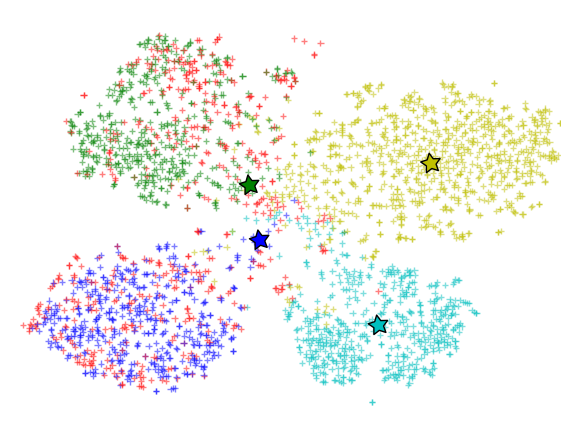
\includegraphics[width=\linewidth]{images/knn}
    % \caption{Signatures mapped to image spacing using Eq. \eqref{eq:dic} and denoted by stars. Then classification done using nearest neighbor}
    \caption{}
\label{fig:knn}
  \end{subfigure}
%
  \begin{subfigure}[b]{0.38\linewidth}
    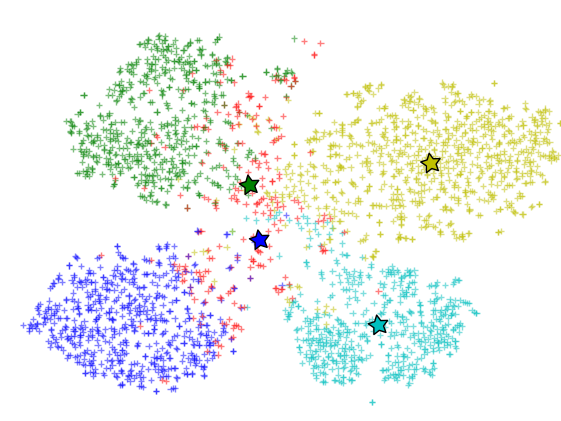
\includegraphics[width=\linewidth]{images/kmeans}
    % \caption{Stars as previous. Classification done by our compatibility function on cluster assignments from k-means}
    \caption{}
\label{fig:kmeans}
  \end{subfigure}
%
  \begin{subfigure}[b]{0.38\linewidth}
    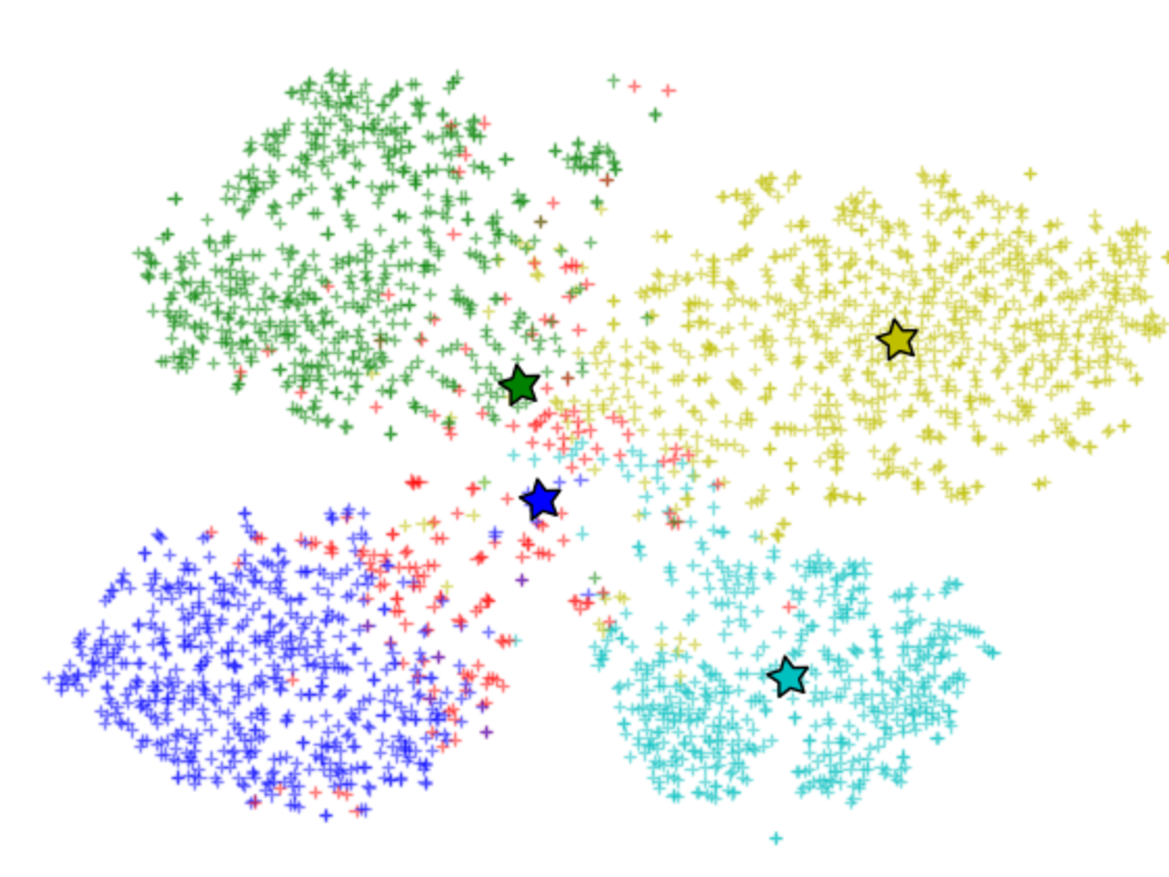
\includegraphics[width=\linewidth]{images/own_cluster}
    \caption{}
    \label{fig:clustering}
% \caption{Stars as previous. Classification by our compatibility function using our supervised clustering}
  \end{subfigure}
%
  \begin{subfigure}[b]{0.38\linewidth}
    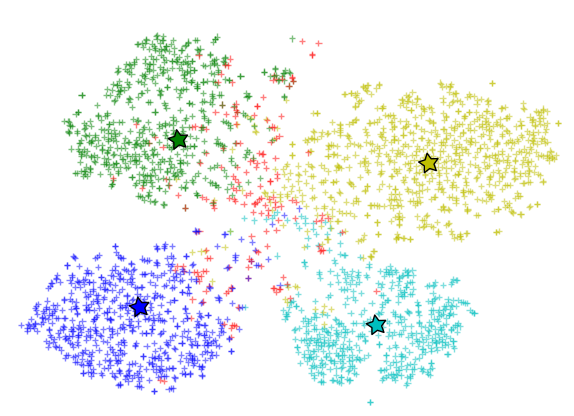
\includegraphics[width=\linewidth]{images/jeac}
    \caption{}
    \label{fig:jeac}
% \caption{Class signatures mapped to image space (stars) and cluster assignment by JEaC}
  \end{subfigure}
  \caption[تحلیل قسمت‌های مختلف روش پیشنهادی]{
  نمایش دوبعدی چهار دسته از مجموعه دادگان AwA با استفاده از نگاشت \lr{t-SNE}، دو دسته‌ی دیده شده شامل بزگوزن (فیروزه‌ای) خرس گریزلی (زرد) و دو دسته‌ی دیده نشده شامپانزه (آبی) و پاندا (سبز). تصاویر با نماد بعلاوه و نگاشت توصیف دسته‌ها در فضای تصاویر با ستاره نشان داده شده است. در تصاویر (ب) تا (و) نقطه‌های قرمز نمونه‌هایی که را نشان می‌دهد که دسته‌ای به جز چهار دسته‌ی موجود در شکل برای آن‌ها پیش‌بینی شده است.
  \textbf{آ)}
   دسته‌های دیده شده با برچسب صحیح و دیده‌نشده با رنگ مشکی
\textbf{ب)}
 نمایش برچسب صحیح برای تمامی دسته‌ها
  \textbf{ج)} توصیف‌ها با نگاشت \eqref{eq:d_answer}
  به فضای تصاویر برده شده‌اند و دسته‌بندی با دسته‌بند نزدیک‌ترین همسایه انجام شده است.
  \textbf{د)}
   نگاشت مانند حالت قبل و دسته‌بندی با تابع مطابقت پیشنهادی به همراه خوشه‌بند \lr{k-means}
  \textbf{هـ)}
   نگاشت مانند حالت قبل و دسته‌بندی با تابع مطابقت پیشنهادی به همراه خوشه‌بند نیمه‌نظارتی پیشنهاد شده
  \textbf{و)}
  دسته‌بندی و نگاشت با استفاده از روش پیشنهادی برای یادگیری نگاشت و خوشه‌بندی توام.
  }
\label{fig:discussion}
\end{figure}

\section{جمع‌بندی}\label{exp:conclusion}
در این فصل نتایج آزمایشات عملی برای روش‌های مختلف پیشنهادی در فصل قبل ارائه شد. ابتدا  مجموعه‌دادگان مورد استفاده معرفی شد. در ادامه
شبکه عصبی چندوظیفه‌ای پیشنهادی مورد بررسی قرار داده شد و نتایج آن با سایر روش‌های پیش‌بینی صفت و هم‌چنین حالت ساده شده که از نمونه‌های آزمون استفاده نمی‌کند مقایسه شد. همچنین تابع مطابقت پیشنهادی به خروجی این شبکه اضافه شد که دقت پیش‌بینی‌های انجام شده را افزایش داد. پس از آن  عمل‌کرد روش خوشه‌بندی نیمه‌نظارتی پیشنهادی مورد بررسی قرار گرفت. هم‌چنین  روش دسته‌بندی  با یادگیری و خوشه‌بندی مجزا و توام مورد آزمایش قرار گرفته و نتایج حاصل از آن‌ها با اخیرترین روش‌های یادگیری بدون نمود نمونه‌ای مقایسه شد. در نهایت  نتایج ارائه شده، مورد بررسی و مقایسه قرار گرفتند و علل عمل‌کرد برتر روش‌های پیشنهادی عنوان شد.
